\documentclass[a4paper,10pt]{article}
\usepackage[utf8]{inputenc}
\usepackage{graphicx}
\usepackage{caption}
\usepackage{subcaption}
\usepackage[left=1.0in, right=1.0in]{geometry}
\usepackage[section]{placeins}

% Alter some LaTeX defaults for better treatment of figures:
    % See p.105 of "TeX Unbound" for suggested values.
    % See pp. 199-200 of Lamport's "LaTeX" book for details.
    %   General parameters, for ALL pages:
    \renewcommand{\topfraction}{0.9}	% max fraction of floats at top
    \renewcommand{\bottomfraction}{0.8}	% max fraction of floats at bottom
    %   Parameters for TEXT pages (not float pages):
    \setcounter{topnumber}{2}
    \setcounter{bottomnumber}{2}
    \setcounter{totalnumber}{4}     % 2 may work better
    \setcounter{dbltopnumber}{2}    % for 2-column pages
    \renewcommand{\dbltopfraction}{0.9}	% fit big float above 2-col. text
    \renewcommand{\textfraction}{0.07}	% allow minimal text w. figs
    %   Parameters for FLOAT pages (not text pages):
    \renewcommand{\floatpagefraction}{0.7}	% require fuller float pages
	% N.B.: floatpagefraction MUST be less than topfraction !!
    \renewcommand{\dblfloatpagefraction}{0.7}	% require fuller float pages


%opening
\title{A Surface LIC algorithm for parallel interactive exploration of large composite datasets}
\author{Burlen Loring}

\begin{document}

\maketitle

\begin{abstract}

\end{abstract}

\section{Introduction}
A composite dataset is simply a dataset organized into a tree of chunks of geometry and coresponding scalar, vector, and tensor fields. Because of their I/O scalability and the simplicity and flexibility in terms of load balancing when the number of visualization process differs from the number of processes used to compute a given simulation, composite datasets are employed ubiqutously in high perfromance parallel scientific data visualization. This work presents a surface LIC algorithm specifically tailored for interactive visualization and exploration of large composite datasets. By designing the parallel load balancing and compositing algorithm specifically for composite data gains in efficiency are attained by redcuing interprocess communication and redundant compuation. 

The effectiveness of surface LIC technique is highly sensative to a number of external parameters such as the choice of surface geometry, the characteristics of the underlying vector field, the user's choie of camera postion, orientation, and other view related paramters, the user's choice of scene lighting, and screen resolution. The effectiveness of the technique is also affected by a number of internal paramters such as the characteristic of the noise used in convolution, and integration parameters such as step size and number of steps taken. By its nature the LIC process inherently reduces dyanmic range of its output. In the limit as the number of convolution steps approaches infinity the LIC output approaches a median(with respect to the input noise) uniform gray scale value. As this limit is approached patterns in the LIC are lost and ability to effecively visualize scalar field by applying color to LIC is diminished. As a user interactively explores a dataset varying any one of these parameters can drasticlly alter the result, thus a great deal of flexibility is needed to provide acceprtable result generally for all values of this paramter space. AUrtomatic and user tunable features that result in excellent results across the paramter space are presented. 

The work presented here has been incorporated into the popular scientific data visualizaiton library VTK. It has also been specifically designed to work with the popular parallel compositing library IceT, so that it may also be used within popular parallel scientific data visualization codes like ParaView and VisIt which both use IceT for image compositing. The work is distributed with ParaView as well.
\FloatBarrier 

\section{Preliminaries}
\subsection{Operations on pixel extents}
\begin{figure}[h]
 \centering
 \includegraphics[width=0.9\textwidth]{./images-data/operations.png}
 % operations.png: 1849x326 pixel, 72dpi, 65.22x11.50 cm, bb=0 0 1849 326
 \caption{Operations on pixel extents. The results of three common operations on the two extents $A$, and $B$, are shown in green. Left, intersection. Center, union. Right, subtraction.}
 \label{fig:pixel-ops}
\end{figure}

When thinking about algorithms designed for rendering parallel composite datasets it's convinient to introduce the concept of a ``pixel extent''. A pixel extent is defined simply as a set of 4 integer values decribing an axis aligned bounding rectangle in screen space. This light weight meta data is useful for describing and manipulating regions ins screenspace. For example we use this abstraction to describe the view and subsets of the view containing valid data for each leaf dataset on each MPI process. Pixel extents are light enough to be quickly communicated to all processes with little overhead making it possible for all processes to know how data is distributed. Additionally, pixel extents are mapped easily to the MPI subarray datatype and thus simplyfy the description of ``zero-copy'' data transfers of non-contiguous regions of memory between processes or locally from one buffer into another. Here the source and destination buffers need not be the same size, or dimensions, but the source and destination extent do. Thus they facilitate transfers of data needed for load balancing and compositing. 

When combined with mathematical operators pixel extents are a powerful abstraction for determining both the cost of and the steps required to composite the vector field. The following set of opertions are useful, sizeof, union($\cup$), intersection($\cap$), shift, merge, and subtract(-). For example in figure \ref{fig:pixel-ops} given two overlaping extents $A$ and $B$, if $A$ and $B$ are on different processes then during compositing the data described by the exent $A \cap B$ must be excahnged between these processes and communication cost of this exchange will be proportional to sizeof$(A \cap B)$.

\subsection{Pipeline}
\begin{figure}[ht]
 \centering
 \includegraphics[width=\textwidth]{./images-data/dia-serial/surfacelic-painter-and-lic2d-flow.png}
 % surfacelic-painter-and lic2d-flow.png: 4131x2242 pixel, 200dpi, 52.46x28.47 cm, bb=0 0 1487 807
 \caption{Logical processing stages}
 \label{fig:flow}
\end{figure}

Here an overview of the pipeline used to compute 

Conceptually our surface LIC algorithm projects vectors defined on an arbitrary surface onto the surface and then from world space into screen space where an image LIC is computed\cite{surfacelic} \cite{imagelic}. When running in parallel the transition from from world space to screen space necessitates a compositing step that gathers pixels to the process that needs them. Because we are implementing our algorithm inside of a larger eco-system, depending on the load balancing algorithm selected a scatter stage that puts pixels back on their original processes may be needed. This step is primarilly dictated by IceT which determines which pixels are touched by a given process and composites only those pixels. Our algorithm is MPI parallel and through GPGPU programming techniques can be accelerated by GPU's where available and threading where GPU's are not available\cite{xsede13}.

A schematic of the algorithm is presented in figure \ref{fig:flow}.This is shown on the left half of the diagram. In this figure, optional processing stages are shaded gray, we show chached textures as red parallelograms, and green double arrows indicate inter-process communication. The major processing stages of the surface LIC are 1) lighting computations and vector projection, 2) a gaurd pixel generation, load balancing, and compositing stage, 3) a stage computing the LIC in image space, 4) A scatter stage to move the data back to where it was prior to compositing; 5) a shading stage that combines image LIC and results of scalar coloring and lighting computations; 6) a color contrast enhancement stage; 7) a stage performing depth test and copying the final result into the default FBO. See appendix \ref{sec:slic-output} for example of output of each stage.

We have split the algorithm into logical processing stages and show them organized in two groups, the vertex processing group(red) and the fragment processing  group(green). During vertex processing we loop over each process's composite data leafs, rendering each to a single texture using a shader that projects vectors, computes lighting, and applies scalar coloring to lit surface geometry. During this stage depth test is enabled which results in a localy correct vector field in image space. To produce the globally correct vector field a compositing stage is employed. Prior to fragment processing we compute the screen space projection, or pixel extent, of each composite dataset leaf's world space axis aligned bounding box. Each leaf's pixel extent is further tightened using the depth buffer and vector field. We then utilize the collection of tight pixel extents to initiate the fragment processing stages by rendering screen aligned quads over just the fragments described be each pixel extent. Limitting fragment processing to tight pixel extents can significiantly reduce the number of fragments that each stage processes for example see section \ref{sec:compsoiting}.

On the right half of the figure a break-out diagram detailing the processing stages used in our image LIC algorithm are shown. Our image LIC algorithm is implemented in two passes. In the first pass, fragments are masked based on user provided criteria\cite{surfacelic} then a basic LIC is computed\cite{imagelic}. In the second pass, the result of the first pass is run through contrast and edge enhancment stages before being used as ``noise'' texture in the second LIC pass. The second pass substantially improves the visual quality of the streaks.  Finally optoinal anti-aliasing and contrast enharncement stages are applied. 

\begin{figure}[ht]
	\centering
	\includegraphics[width=0.9\textwidth]{./images-data/dia-serial/lg-lic2d-200ppi.png}
	% lic2d-flow.eps: 0x0 pixel, 300dpi, 0.00x0.00 cm, bb=0 0 610 807
	\label{fig:lic2d-outputs}
  \caption{Line integral 2D stages}
\end{figure}

\FloatBarrier

\section{Features for interactive data exploration}
\begin{figure}[ht!]
 \centering
 \includegraphics[width=0.9\textwidth]{./images-data/dia-serial/color-ce-curves-khB-both-h.png}
 % color-ce-curves-khB-both.png: 2175x2441 pixel, 72dpi, 76.72x86.10 cm, bb=0 0 2175 2441
 \caption{Improving the transfer of scalar coloring via contrast enhancement stages. The top pannels show visualization of surface LIC of magentic field on a slice colored by magnetic field and the RGB color curves for the image. The bottom pannels show the same visualization but using the contrast enhencement stages. The contrast enhancement improves the effectiveness of the scalar coloring and LIC in the resulting image.}
 \label{fig:cce-khb}
\end{figure}
What characteristics in the output LIC make for an effective visualization across a wide variety of input data and rendering conditons? Some of the important characteristics in an effective surface LIC visualizaion are
\begin{enumerate}
 \item The LIC patterns accurately represent the characteristics of the underlying vector field. If desired the relative strength and features in strongly vearying fields should be maintained.
 \item When scalar coloring is desired, LIC pattern must not be lost during the application of colors and similarly scalar colors once applied should not be dull or have greatly diminished intensity.
 \item Over all a high dynamic range in the resulting image is desirable. This make it easy to identify feature in LIC and scalar colors. The lower the dyanmic range the less decernable detail there is in the result.
 \item Lighting characteristics must be maintained, for example shadows, specular reflections, etc.
 \item The algorithm should perform well on very large surface geometry
\end{enumerate}

\subsection{Scalar color shading}
When thinking about how best to acheive these goals it's important to consider how scalar colored, lit geometry and and image LIC are combined to produce the final result. In our algorithm scalar coloring and lighting caclulations are rendered and stored in a texture. The image LIC is computed using projected vectors and also stored in a texture. There are two common approaches for combining these two textures into the final resut, a multiplciative or mapping approach\cite{image-lic} and an addative or blending approach\cite{surface lic}.

The mapping approach is described by the following equation:
\begin{equation}
c_{ij} = ( L_{ij} + f ) * S_{ij}
\label{eqn:color-map}
\end{equation}
where the indices $i,j$ identify a specific fragment, $c$ is final RGB color, $L$ is LIC gray scale intensity, $S$ is the scalar RGB color, and $f$ is a biasing parameter, typically 0, that may be used for fine tuning. When $f=0$, the typical case, colors are transfered directly to the final image where the LIC is 1, and a linearly scaled transfer of scalar colors where LIC gray scale color is less than one down to 0, where the final color is black. The bias parameter $f$ may be set to small positiver or negative values between -1 and 1 to increase or decrease LIC values uniformly resulting in brighter or darker images. When $f\neq0$ final fragment colors, $c$, are clamped such that $0 \leq c \leq 1$.

With the mapping approach the distribution of intensity values in the LIC directly affect the accuracy and intensity with which scalar colors and lighting effects are transfered to the final result and the average brightness and contrast of the result. Note in the final result that individual RGB channel values will be less then or equal to the maximum grayscale value in the image LIC. Also, the greater the number of pixels close to 1 in the image LIC, the more acurately and intensly scalar coloring and lighting are transfered into the final image. However, this must be balanced with a sufficient number of highly contrasting pixels where the value is closer to 0 in order to accurately represent the LIC pattern. Put sucintly it's critical that the image LIC has high contrast and dynamic range with a good mix of light and dark values if it is to be effectively mapped onto scalar colors. However, the convolution process inheriently reduces both contrast and dynamic range in the image LIC. To correct this we've introduced contrast enhancment stages in three places in the pipeline. An example demonstrating the effectiveness of the contrast enhancement stages is shown in figure \ref{fig:cce-khb}. The top


The blending approach for combining scalar colors, lighting effects, and the image LIC is described by the following equation:
\begin{equation}
c_{ij} = L_{ij} * I + S_{ij} * (1 - I)
\label{eqn:color-blend}
\end{equation}
where the indices $i,j$ identify a specific fragment, $c$ is final RGB color, $L$ is LIC gray scale value, $S$ is the scalar RGB color, and $I$ is a constant ranging from 0 to 1, with a default of 0.8. Decreasing $I$ to obtain brighter colors diminishes the intensity of the LIC, and vise versa. When colors are bright the LIC is difficult to see. Currently, the best results are obtained by sacrificing slightly on both fronts. The blending approach bennefits from an image LIC with high contrast and dyanmic range as this tends to make patterns in the image LIC more easily visible after blending. Note that despite the fact that it inheriently decreases visibility of features in scalar coloring and image LIC, the blending approach is especially useful with curved surfaces and pronounced lighting effects and also when scalar color map is very intense.
\FloatBarrier

\subsection{Contrast enahancement}
\label{sec:contrast}
\begin{figure}[h!]
 \centering
\begin{subfigure}{0.48\textwidth}
\includegraphics[width=\textwidth]{./images-data/dia-serial/gray-ce1-curves.png}
% gray-ce1-curves.png: 1187x1078 pixel, 200dpi, 15.07x13.69 cm, bb=0 0 427 388
\caption{}
\label{fig:gray-ce-curves1}
\end{subfigure}
\hspace{0.15in}
\begin{subfigure}{0.48\textwidth}
\includegraphics[width=\textwidth]{./images-data/dia-serial/gray-ce2-curves.png}
% gray-ce1-curves.png: 1187x1078 pixel, 200dpi, 15.07x13.69 cm, bb=0 0 427 388
\caption{}
\label{fig:gray-ce-curves2}
\end{subfigure}
\begin{subfigure}{0.48\textwidth}
\centering
\includegraphics[width=\textwidth]{./images-data/dia-serial/color-ce-curves.png}
% gray-ce1-curves.png: 1187x1078 pixel, 200dpi, 15.07x13.69 cm, bb=0 0 427 388
\caption{}
\label{fig:gray-ce-curves2}
\end{subfigure}
\caption{}
\end{figure}

The convolution process tends to decrease both contrast and dynamic range, often producing dark and dull results. Figure \ref{fig:motivation}.a illustrates this issue. The narrowing of dynamic range and diminishing of contrast are consequences of the convolution operation which convolves a noise texture with a vector field. These reductions are made worse by the use of  Gaussian noise because by definition centrally concentrates its values about a mid gray tone.

In order to counteract this, optional contrast enhancement stages have been added. The new stages increase the dynamic range and contrast without modifying the patterns that emerge from the LIC process or modifying the scalar colors. VTK's surface LIC implementation is provided by two classes, the vtkSurfaceLICPainter and vtkLineIntegralConvolution2D. The vtkSurfaceLICPainter, projects vectors, sets up noise texture, and passes control to the vtkLineIntegralConvolution2D to generate a LIC, after which it shades scalar colors combined with the generated LIC onto the surface geometry. Contrast enhancement stages have been added to both classes.


% \subsection{vtkLineIntegralConvolution2D}
The contrast enhancement stages are implemented by histogram stretching of the gray scale colors in the LIC'ed image as follows:
\begin{equation}
c_{ij} = \frac{c_{ij} - m}{M - m}
\end{equation}
where, the indices $i,j$ identify a specific fragment, $c$ is the fragment's gray scale color, $m$ is the gray scale color value to map to 0, $M$ is the gray scale color value to map to 1. When the contrast enhancement stage is applied on the input of the high-pass filter stage, $m$ and $M$ are always set to the minimum and maximum gray scale color of all fragments. In the final contrast enhancement stage $m$ and $M$ take on minimum and maximum gray scale colors by default but may be individually adjusted by the following set of equations:
\begin{equation}
m = min(C) + F_{m} * ( max(C) - min(C) )
\end{equation}
\begin{equation}
M = max(C) - F_{M} * ( max(C) - min(C) ) 
\end{equation}
where, $C = \{c_{00},c_{01},...,c_{nm}\}$, are all of the gray scale fragments in the LIC image and $F_m$ and $F_M$ are adjustment factors that take on values between 0 and 1. When $F_m$ and $F_M$ are 0 minimum and maximum are gray scale values are used. This is the default. Adjusting $F_m$ and $F_M$ above zero controls the saturation of normalization. This is useful, for example, if the brightness of pixels near the border dominate because these are convolved less because we can't integrate outside of the dataset.

Occasionally, often depending on the contrast and dynamic range and graininess of the noise texture, jagged or pixelated patterns may emerge in the LIC. These can be reduced by enabling the optional anti-aliasing pass.

% \subsection{vtkSurfaceLICPainter}
The color contrast enhancement stage is implemented with histogram stretching on the fragments lightness in the HSL color space.
\begin{equation}
L_{ij} = \frac{L_{ij} - m}{M - m}
\end{equation}
where, the indices $i,j$ identify a specific fragment, $L$ is the fragment's lightness in HSL space, $m$ is the lightness to map to 0, $M$ is the lightness to map to 1. $m$ and $M$ take on minimum and maximum lightness over all fragments by default but may be individually adjusted by the following set of equations:
\begin{equation}
m = min(L) + F_{m} * ( max(L) - min(L) )
\end{equation}
\begin{equation}
M = max(L) - F_{M} * ( max(L) - min(L) ) 
\end{equation}
where, $L$ are fragment lightness values and $F_m$ and $F_M$ are the adjustment factors that take on values between 0 and 1. When $F_m$ and $F_M$ are 0 minimum and maximum are lightness values are used. This is the default. Adjusting $F_m$ and $F_M$ above zero provides fine-tuning control over the saturation.

\FloatBarrier

\subsection{Noise generator}
\begin{figure}[ht]
 \centering
 \includegraphics[width=0.9\textwidth]{./images-data/dia-serial/ensight-blow-multiblock-frame.png}
 % ensight-blow-multiblock-frame.png: 1414x1074 pixel, 72dpi, 49.88x37.88 cm, bb=0 0 1414 1074
\caption{Visualizations demonstrating affect of varying noise texture and scalar color shader. An Ensight Multi-Block dataset from a simulation of shell being crushed is used.
    {\bf (a)} Blending scalar color shader, solid color.
    {\bf (b)} Mapping scalar color shader, solid color.
    {\bf (c)} Mapping scalar color shader, a custom noise texture (Gaussian, grain size 1), and contrast enhancement.
    {\bf (d)} Blending scalar color shader, color by scalars.
    {\bf (e)} Mapping scalar color shader, color by scalars.
    {\bf (f)} Mapping scalar color shader, color by scalars, a custom noise texture (Perlin, grain size 4), and contrast enhancement.}
 \label{fig:noise}
\end{figure}

Important factors in determining the characteristcs of streaking patterns in the LIC and in overall contrast and dynamic range of the final image are the characteristics of the noise to be convolved with the vector field. By varying the properties of the noise input into the image LIC algorithm one gains much control over the output. Using the same noise texture produces markedly different results on different datasets and even on the same dataset at different screen resolutions. A single noise texture will not work well in all cases. Thus a run time tunable noise texture generator is a key component in our algoirthm. 

Our noise texture generator defines the following 9 run time modifiable degrees of freedom, we have found that these 9 paramters are highly effective for controlling streaking pattern, dynamic range, and contrast, in in the resulting LIC.
\begin{description}
\item[Noise type] This parameter controls the underlying statistical distribution of values in the generated noise texture, or type of noise generated. The user may choose from Gaussian noise, uniformly distributed noise, or Perlin noise. By default Gaussian noise is used.
\item[Texture size] This paramter controls the size of the square noise texture in each direction. Support for non-power of 2 textures is assumed. However in the case of Perlin noise the texture size is adjusted to the nearest power of 2.
\item[Grain size] Select the number of pixels  in each direction that each generated noise element fills in the resulting texture. For Perlin noise this sets the size of the largest scale, and must be a power of 2.
\item[Min value] This parameter sets the lowest gray scale value realizable in the generated noise texture. This paramter can range between 0 and 1 and the default value is 0.
\item[Max value] This parameter sets the highest gray scale value realizable in the generated noise texture. This paramter can range between 0 and 1 and the default value is 0.8.
\item[Number of levels] Set the number of realizable gray scale values. This parameter can range from 2 to 1024 and the default value is 1024.
\item[Impulse probability] This parameter controls how likely a given element is to be assigned a value. When set to 1 all elements are filled. When set to some number lower than one a fraction of the texture's elements are filled with generated noise. Elements that are not filled take on a background color value. The default impulse probablity is 1.
\item[Background color] The gary scale value to use for un-touched pixels when the impulse probability paramter is set less than 1. The default background value is 0.
\item[RNG seed] Modify the seed value of the random number generators.
\end{description}
Changing the noise texture gives one greater control over the look of the final image. For example, with impulse noise by varying the impulse probability along with the choice of background intensity control over number of light or dark pixels in the LIC image is attained. This greatly helps the transfer of patterns in scalar coloring and lighting to the final image. Varying the noise grain size along with impulse probabilty and impulse background back color give greater control over the width of the streaks generated by the image LIC stage. With the ability to selecting a noise distribution, its minimum, maximum, and number of noise levels, control over the contrast is gained. 
\FloatBarrier

\subsection{Integrator Normalization}
\begin{figure}[htpb]
 \centering
 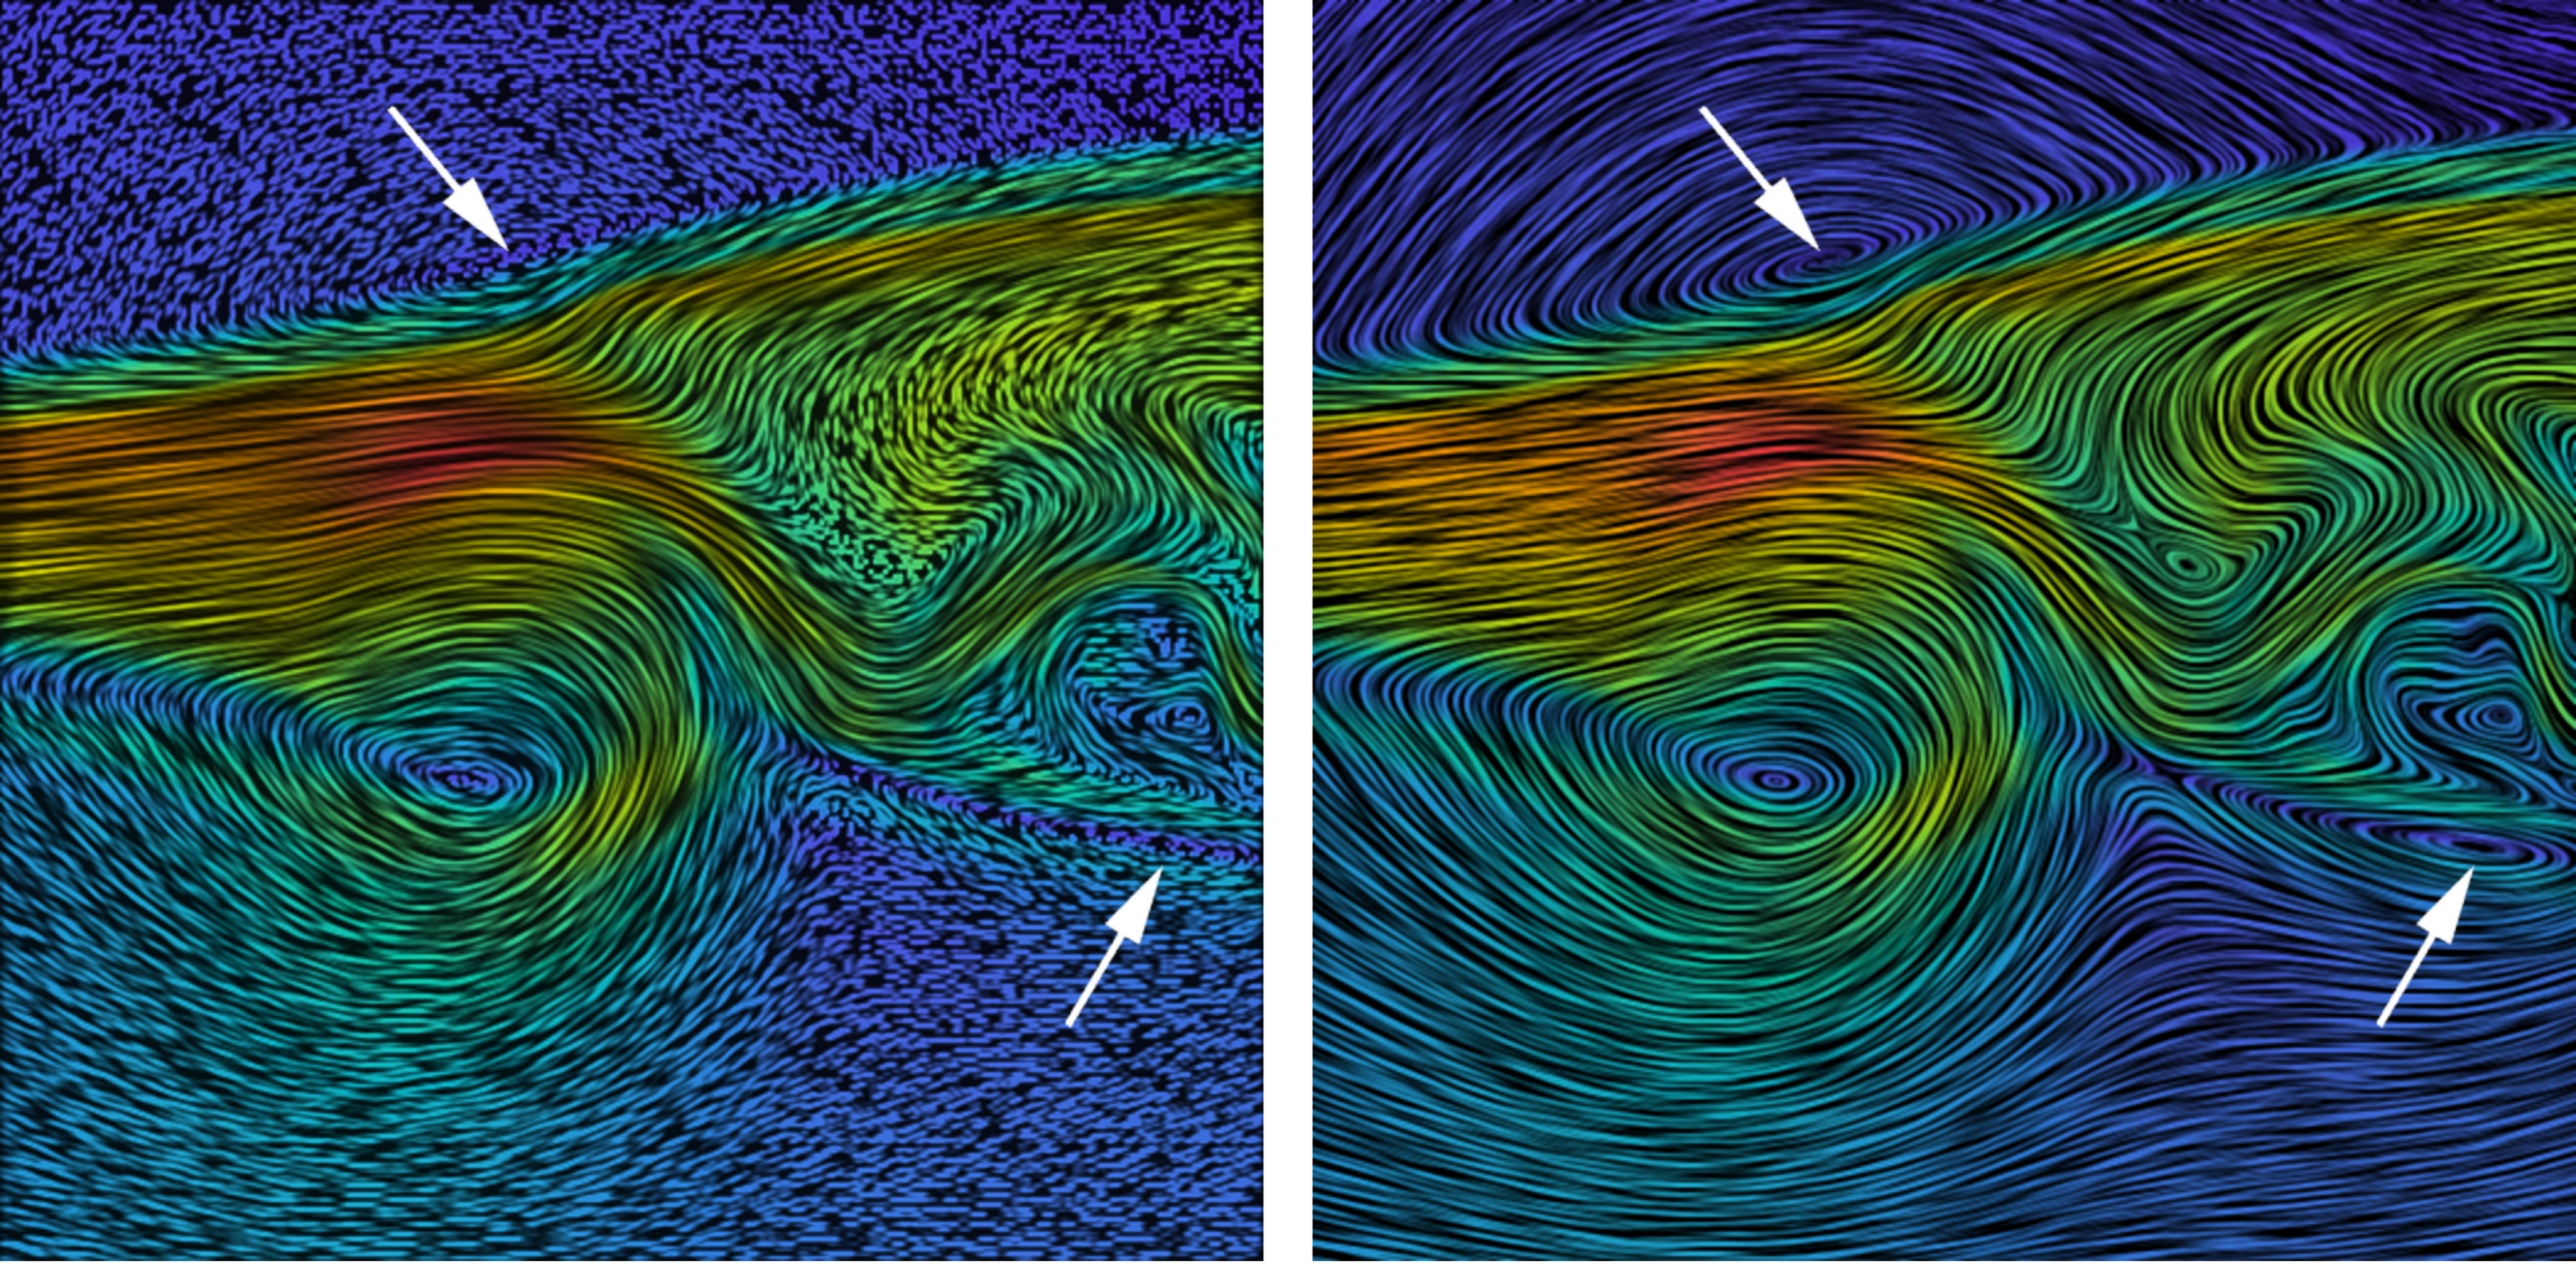
\includegraphics[width=\textwidth]{./images-data/vector-norm/vec-norm.png}
 % vec-norm.png: 2100x1028 pixel, 72dpi, 74.07x36.26 cm, bb=0 0 2100 1028
 \caption{vector normal}
 \label{fig:vec-norm}
\end{figure}

Normalizing vectors during integration is a trick that can be used to simplify integrator configuration and give the resulting LIC a uniformly smooth look. By using normalized vector field values the convolution occurs over the same integrated arclength for all pixels in the image. This gives the result a smooth and uniform look and makes it possible to provide reasonable default values for step size and number of steps to the integrator independent of the input vector field. The resulting visualization acurately shows the tangent field however variations in the relative strength of the vector field is lost and can alter the relationships of flow features making weak features prominent and strong features less so. In the context of developing a general puprose tool for interactive data exploration it's important to provide both options and let the user select the option that best fits her needs. For example figure \ref{fig:vec-norm} shows the result of the algorithm applied to a simulation of magnetic reconnection in a hot plasma with and without integrator normalization. In this case normalization can give a false sense of the importance of a number of flow features.

% \subsection{Fragment Masking}
% \label{sec:mask}
% Currently the criteria for masking fragments is that all vector components must be identically zero. This doesn't work for many numerical simulations where stagnant flow is not identically zero due to numerical rounding. For example, stagnate flow might be where $|V|<1e^{-6}$. Also, the lack of control over the color characteristics of the masked fragments result in masked fragments looking drastically different than the LIC'ed fragments. This is illustrated in figure \ref{fig:motivation}.d where all fragments on the outer walls have been masked , the masked fragments are much brighter than the the LIC'ed fragments.
% 
% New fragment masking implementation makes use of a user specified threshold value below which fragments are masked. The masking test may be applied either to the original vectors or the surface projected vectors. By applying the test to the original vectors the masked fragments will match scalar colors when coloring by $|V|$. 
% 
% Fragments where $|V|<t$ are masked. The fragment masking implementation provides control over the intensity and color of the masked fragments via the following equation:
% \begin{equation}
% c_{ij} = M * I + S_{ij} * ( 1 - I )
% \label{eqn:color-blend}
% \end{equation}
% where the indices $i,j$ identify a specific fragment, $c$ is final RGB color, $M$ is the RGB mask color, $S$ is the scalar RGB color, and $I$ is the mask color intensity. This allows one control over the masking process so that masked fragments may be: highlighted (by setting a unique mask color and mask intensity > 0), made invisible with and without passing the un-convolved noise texture (by setting mask intensity 0), or made to show the scalar color at a similar level of intensity as the LIC (mask intensity > 0).

% \subsection{Optimizations for interactivity}

\section{Parallelization}
\begin{figure}[ht]
 \centering
 \includegraphics[width=\textwidth]{./images-data/dia-serial/shuttle-surf-par-lg-p-d-space-lic.png}
 % shuttle-surf-par-lg-p-d-space.png: 1702x514 pixel, 72dpi, 60.04x18.13 cm, bb=0 0 1702 514
 \caption{Left: LIC colored by momentum on a surface extracted from composite dataset simulating a launch vehicle\cite{nasa-shuttle} with world space axes aligned bounding boxes colored by dataset id. Center: Screen space projection of the composite dataset's axis aligned bounding boxes colored by MPI process id in a 4 way parallel run. For reference composited vector field colored by magnitdue is shown. The comm cost for this decomposition is 1.8. Right: Pixel extents from the in-place disjoint domain decomposition used to compute the LIC colred by MPI process id with the LIC blended for reference. The comm cost for this decomposition is 0.32.}
 \label{fig:blocks}
\end{figure}
In order to handle datasets larger than can fit on a single compute node the algorithm must be parallelized. In VTK the data partitioning mechanisms are abstracted into the pipeline and away from the rendering algorithm. Therefore, to be compatible with VTK's data parallel pipeline the algorithm must be data parallel where each MPI process is expected to process a subset of the data without access to the remainder of the whole dataset. The surface LIC algorithm is unique compared to other parallel rendering algorithms. First, in the data parallel setting the integration step may require access to off process vector data. We deal with this by adding a gaurd pixel halo to each composite leaf dataset's screen space pixel extents. Additionally, after being projected to screen space and depth test applied ensuring that vector field is correct locally, the vector field must be composited so to ensure correct field values are accessed where there is screen space overlap on multiple processes. 

The parallel rendering algorithm must also take into account the fact that the entirety of the screen space may be, as in the case of large tile displays, too large to fit in the memory of a single process, and take into account the specific requirements of the image compositing engine. For example IceT will compute the union of screen space extent of all the data on each MPI rank and it will only composite from those regions of the screen. Therefor to work seamlessly with IceT each rendering process must update only the pixles that fall within these bounds and no others. This arangement is challenging since depending on the upstream partitioning of data and the view parameters, such as camera position and view frustum definition, in screen space data and work may be distributed unevenly. This also places some restrictions on what load balancing schemes will be practical since any reorganization of screen space data moving data from the intial decompositon to a more favoroable one must then must move it back after the computation has been made adding some communication overhead. When attempting to load balance rendering computations in this environment the goal of acheiving equal distribution of work must be balanced by the compositing and communication costs.

Figure \ref{fig:blocks} shows the situation when rendering the shuttle data, an 8 leaf composite dataset, in parallel on 4 MPI processes. In the left panel the surface LIC is shown along with world space axis aligned bounding boxes. In the center the screen space projection of each world space bounding box is shown colored by MPI rank. Because of the large amount of overlap in screen space this distribution of data will have a high compositing cost as overlapping regions must be exchanged among all processes that have overlap. Additionally overlapping pixels represent redundant computation. On the right, a screen space domain decomposition that minimizes compositing overhead and compution is shown.

\subsection{Gaurd pixel generation}
To ensure correct parallel results of the image LIC computation prior to compositing guard pixel halos are added to compute pixel extents. The number of gaurd pixels required is determinied by the longest arc length of the integration on each pixel extent. When integrator noramlization is used the same across all pixel extents and is given by:
\begin{equation}
n_g = \max( n_s \delta n_p \alpha,  2)
\label{eqn:gaurd-norm}
\end{equation}
where, $n_g$ is the number of gaurd pixels required, $n_s$ is the number of steps to integrate, $\delta$ is the step size, $n_p$ is the number of image LIC passes (either 1 or 2), and $\alpha$ is an addative factor that compensates for beleding at the view edges where it's impossible to compute all $n_s$ steps because guard pixel data is unavailable. At least $2$ guard pixels are employed because linear texture fetches use a texels 4 nearest neighbors.

Note that in \ref{eqn:guard-norm} because vector field is normalized $n_s \delta$ is the arc length of the integration. Without integrator normalization the contribution of the vector field magnitude to the integrated arc length must be accounted for. An upper bound on field strength is required. One complication is that for a given pixel extent the maximum value on that extent may change as a result of compositing the data from the overlaping extents from other processes. This is solved for each extent by finding the maximum on itself and all overlapping extents. Note, that although we don't have the vector field defined on the set of comute extents, it is this set of extents that must be used. This is handled by searching for the maximum value inside the interesction of each overlaping rendering and compute extent.
\begin{equation}
n_g^i = \max(n_s \delta n_p \alpha \max(\mathbf{E} \cap E_i), 2)
\label{eqn:gaurd}
\end{equation}
where, $n_g$ is the number of gaurd pixels required for extent $i$, $E$ is a set, with members consisting of vector field data defined on each extent of the LIC computational domain, and $E_i$ is the extent to compute the number of gaurd pixels for.
\FloatBarrier

\section{Compositing and load balancing strategies}
The per process rendering cost of the vertex and fragment processing stages is typically proportional to the number of vertices per process rendered. With data parallelism, if we assume reasonable data partioning, these costs can be reduced simply by adding parallel processes. However, with this surface LIC algorithm the cost of compositing screen space vectors is a limiting factor. An estimate of the compositing cost associated with moving one screen space domain decomposition, the source decompositon, to another, the destination decomposition, is given the following equation.
\begin{equation}
c = \sum\nolimits_{i=1}^{n_p} \sum\nolimits_{j=1}^{n_l(i)} \sum\nolimits_{p=1,p \neq i}^{n_p} \sum\nolimits_{q=1}^{n_l(p)} \frac{ size(S_{ij} \cap D_{pq}) }{ size(V) }
\label{eqn:comm-cost}
\end{equation}
where, $n_p$ is the number of processes in the parallel job, $n_l(i)$ is the number of composite leaf datasets on process $i$, $S_{ij}$ is the source pixel extent on process $i$ for composite data leaf $j$ currently containing vector data, $D_{ij}$ is the destination pixel extent on process $i$ for compute extent $j$ to receive vector data, the $\cap$ operator takes the intersection of two pixel extents, prodicing exactly the overlapping region between the two, and $size(E)$ operator computes the number of pixels in pixel extent $E$, $V$ is the pixel extent of the view. In plain english this equation says that the cost of compositing is proportional to the number of off process overlaping pixels. This equation provides a means for comparing the cost of compositing to different domain decompositions.  We use this equation at run time to select the best domain decomposition between a number of alternatives. When comparing domain decomposition lower values of $c$ indicate reduced work, thus domain decomposition with the lowest value should be selected. Note that this equation describes the exchange of data, so for example both $A \cap B$ and $B \cap A$ are counted.

The first step in the surface LIC algorithm is to project the vector field into screen space. During the projection step the depth test is applied ensuring that locally correct screen space evctors are selected. Screen space vectors from all composite data leaves are stored in the red and green components of a single floating point texture. Depth buffer values are stored in the alpha channel of this texture for use in compositing. Our compositor makes use of pixel buffer objects PBOs for ``zero copy'' MPI non-blocking interprocess communication of data from remote overlapping regions. Because pixel extents generated by projecting world space axis aligned bounding boxes into screen space are often larger than the actual screen space extent of the rendered data, prior to compositing the vector texture is mapped into CPU memory using a PBO and a pass over each composite data leaf's pixel extent is made to shrink it down to minimal size based on depth buffer values. This tightening of pixel extents reduces compositing overhead and because the compositor requires that the vector texture be mapped into CPU memory for communication the tightening pass incurs the relatively small cost of looping over the depth values. For example the top row of figure \ref{fig:compositing} shows the axis aligned world space bounding boxes and their tight screen space projections for a zoomed in region of the shuttle dataset. The second row of this figure shows the sate of the vector field which is locally correct after projection and depth test, but not gloabally correct. Before computing the LIC in screen space this data must be composited onto the computation domain.

The second step in the surface LIC algorithm is compositing the locally correct screen space projected vectors. At this point that we have the oportunity to choose a screen space domain decomposition on which to compute the image LIC. The careful selection of a domain decompostion on which to compute the image LIC can reduce compositing cost, reduce communications, eliminate redundant computation, and load balance the computation. We have investigated 3 domain decomposition stragtegies and developed a model for estimating the compositing cost so that our surface LIC algorithm will automatically select between them choosing the most efficient. The final three rows in the figure \ref{fig:compositing} show the result of compositing the vector field using one of the domain decompositono strategies. In rows 1 through 5 the first column shows the screen space domain decompositon that the LIC will be computed on. The remaining columns 2 through 5 show the composited vector field for each one of 4 MPI processes. The compositing cost $c$ computed using equation \ref{eqn:comm-cost} is given for each decomposition.
\begin{figure}[t!]
 \centering
 \includegraphics[width=0.9\textwidth]{./images-data/compositing-2-200ppi.png}
 % compositing-200ppi.png: 4269x6208 pixel, 200dpi, 54.22x78.84 cm, bb=0 0 1537 2235
 \caption{Worked example of 4 way MPI parallel rendering of a zommed in region of the shuttle composite dataset(8 leafs) demonstrating 3 compositing strategies.}
%  {\bf row 1} Left: World space axes aligned block bounds and the coresponding screen space extents. Right: Surface LIC rendering.
%  {\bf row 2-5, column 1} Screen space extents for each decomposition colored by process id.
%  {\bf row 2-5, columns 2-5} Rendering showing screen space vector data with one column for each process. Data for each leaf is shown with its coresobonding pixel extent.
%  {\bf row 2} Locally correct projected vectors. This is the input to all compositing strategies.
%  {\bf row 3} In-place decomposition and composited vectors.
%  {\bf row 4} In-place disjoint decomposition and composited vectors.
%  {\bf row 5} Ballanced decomposition and composited vectors.}
 \label{fig:compositing}
\end{figure}

\subsection{In-place strategy}
Given that to work seamlessly with IceT each process is restricted to updating the specific region of screen space defined by the projection of the union of the local composite data leafs a natural approach is to composite the vector field on the this decomposition. Because the domain decomposition is unchanged we call this the ``in-place'' approach. When evaluating the compositing cost of the in-place strategy using equation \ref{eqn:comm-cost} $S$ and $D$ are the same set of extents. One might hope that the world space domain decomposition, which we assume is reasonably load balanced, when projected onto screen space will also be a resonabe choice. This is sometimes the case. For example the in-place approach is optimal when there is no overlap of screen space extents between processes, as in the case of computing the surface LIC on a slice through a composite dataset with exactly one leaf dataset per process. However, for surface geometries with a large degree of sceen space overlap the approach has a relatively high compositing compared to other domain decomposition strategies. One disadvantage of the in-place strategy is that screen space overlap in the compute domain results in the image LIC being computed redundantly on multiple processes. As the results of the benchmark and scaling runs presented in the next section show, this redundant computation is a significant factor in overall performance. An example of compositing using the in-place decomposition is shown in figure \ref{fig:compositing} in row 3. Comparing the decomposition by process readily illustrates the large degree of redundant computation that will occur for this example. 

\begin{figure}[ht]
	\centering
	\begin{subfigure}{\textwidth}
		\centering
		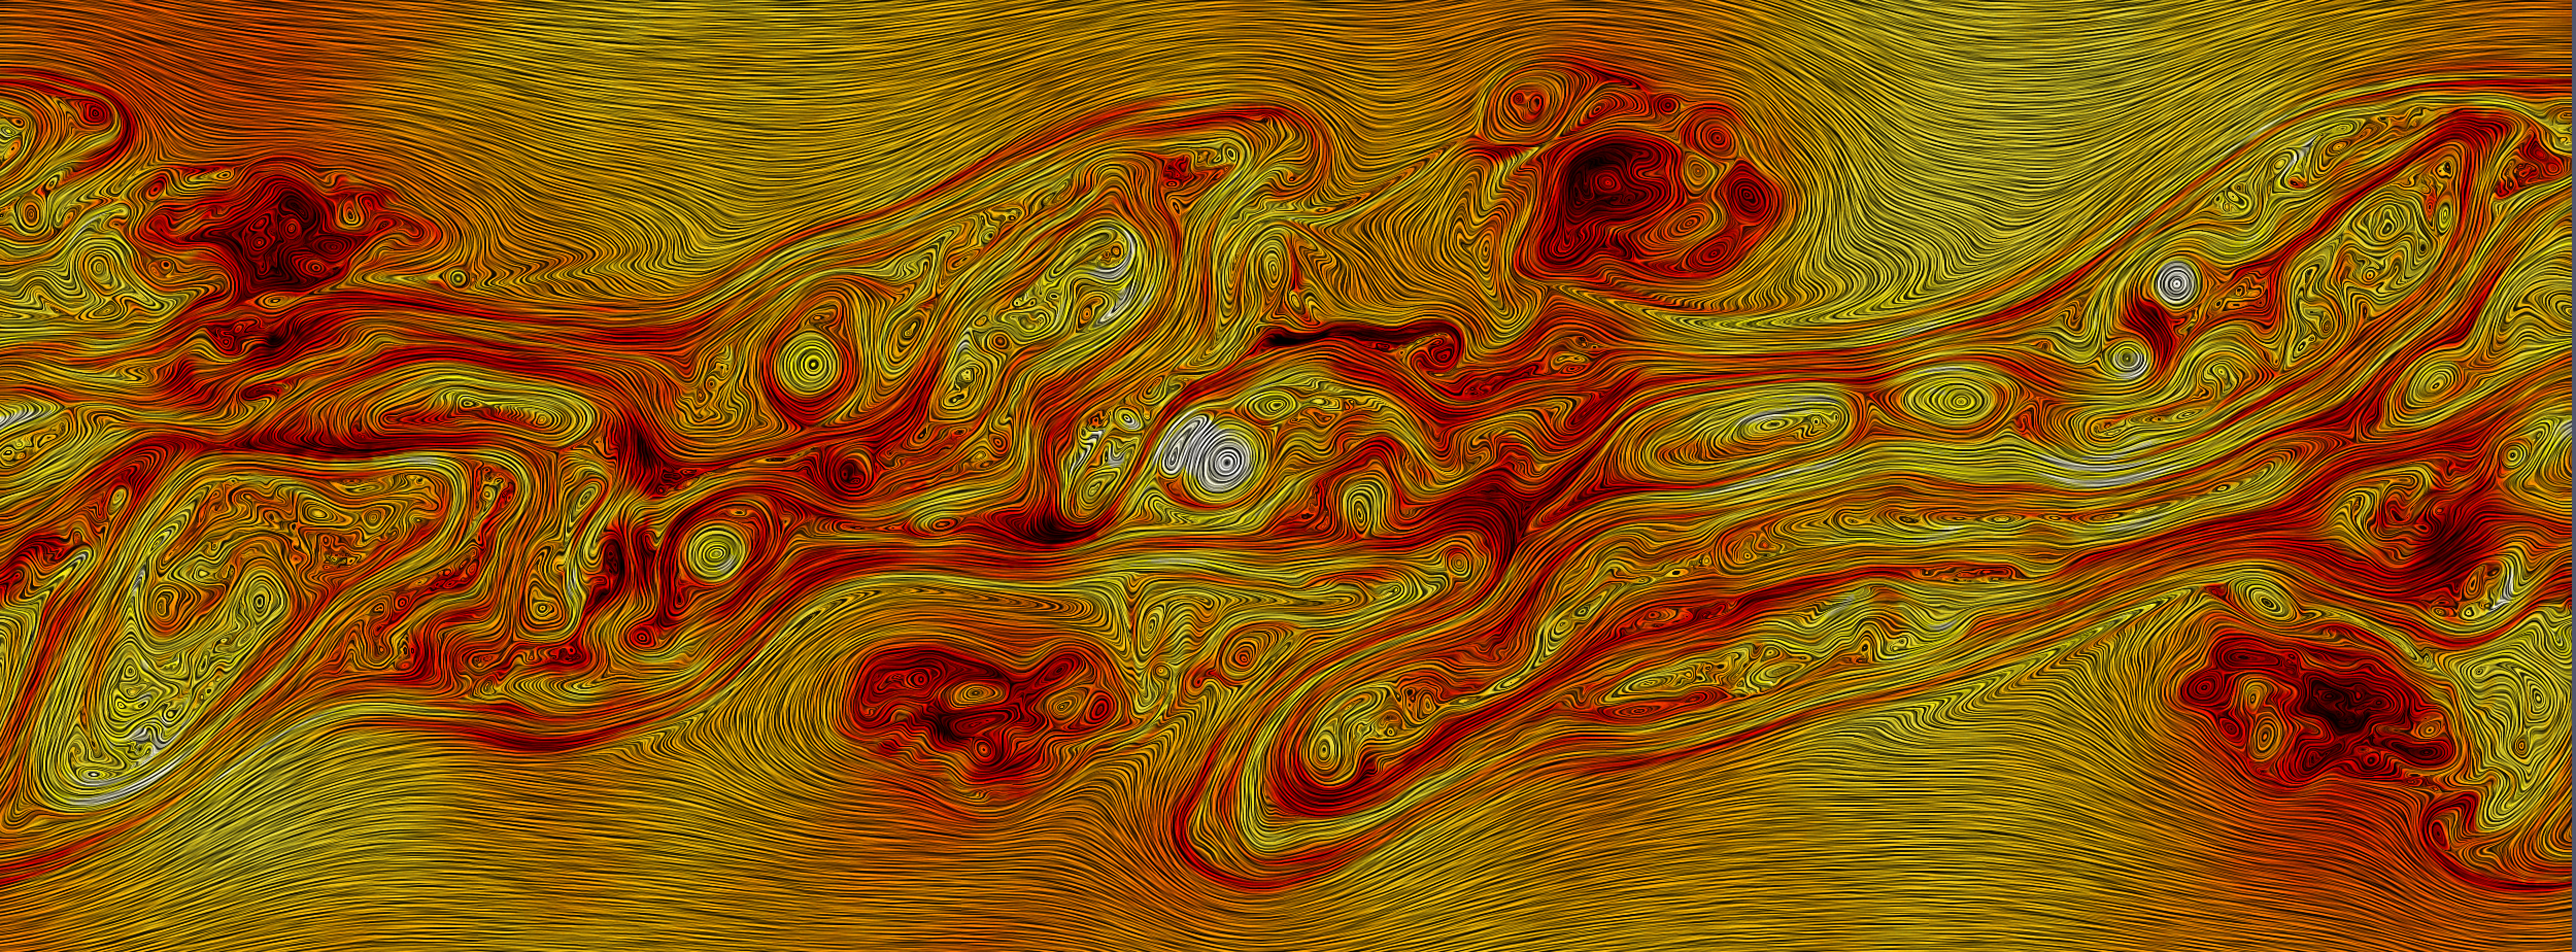
\includegraphics[width=\textwidth]{./images-data/dia-serial/lic-b-427-hr.png}
		% lic-b-427-hr.png: 5000x1848 pixel, 72dpi, 176.37x65.19 cm, bb=0 0 4999 1848
		\label{fig:scaling-lic}
  \end{subfigure}
	\begin{subfigure}{0.5\textwidth}
		\centering
		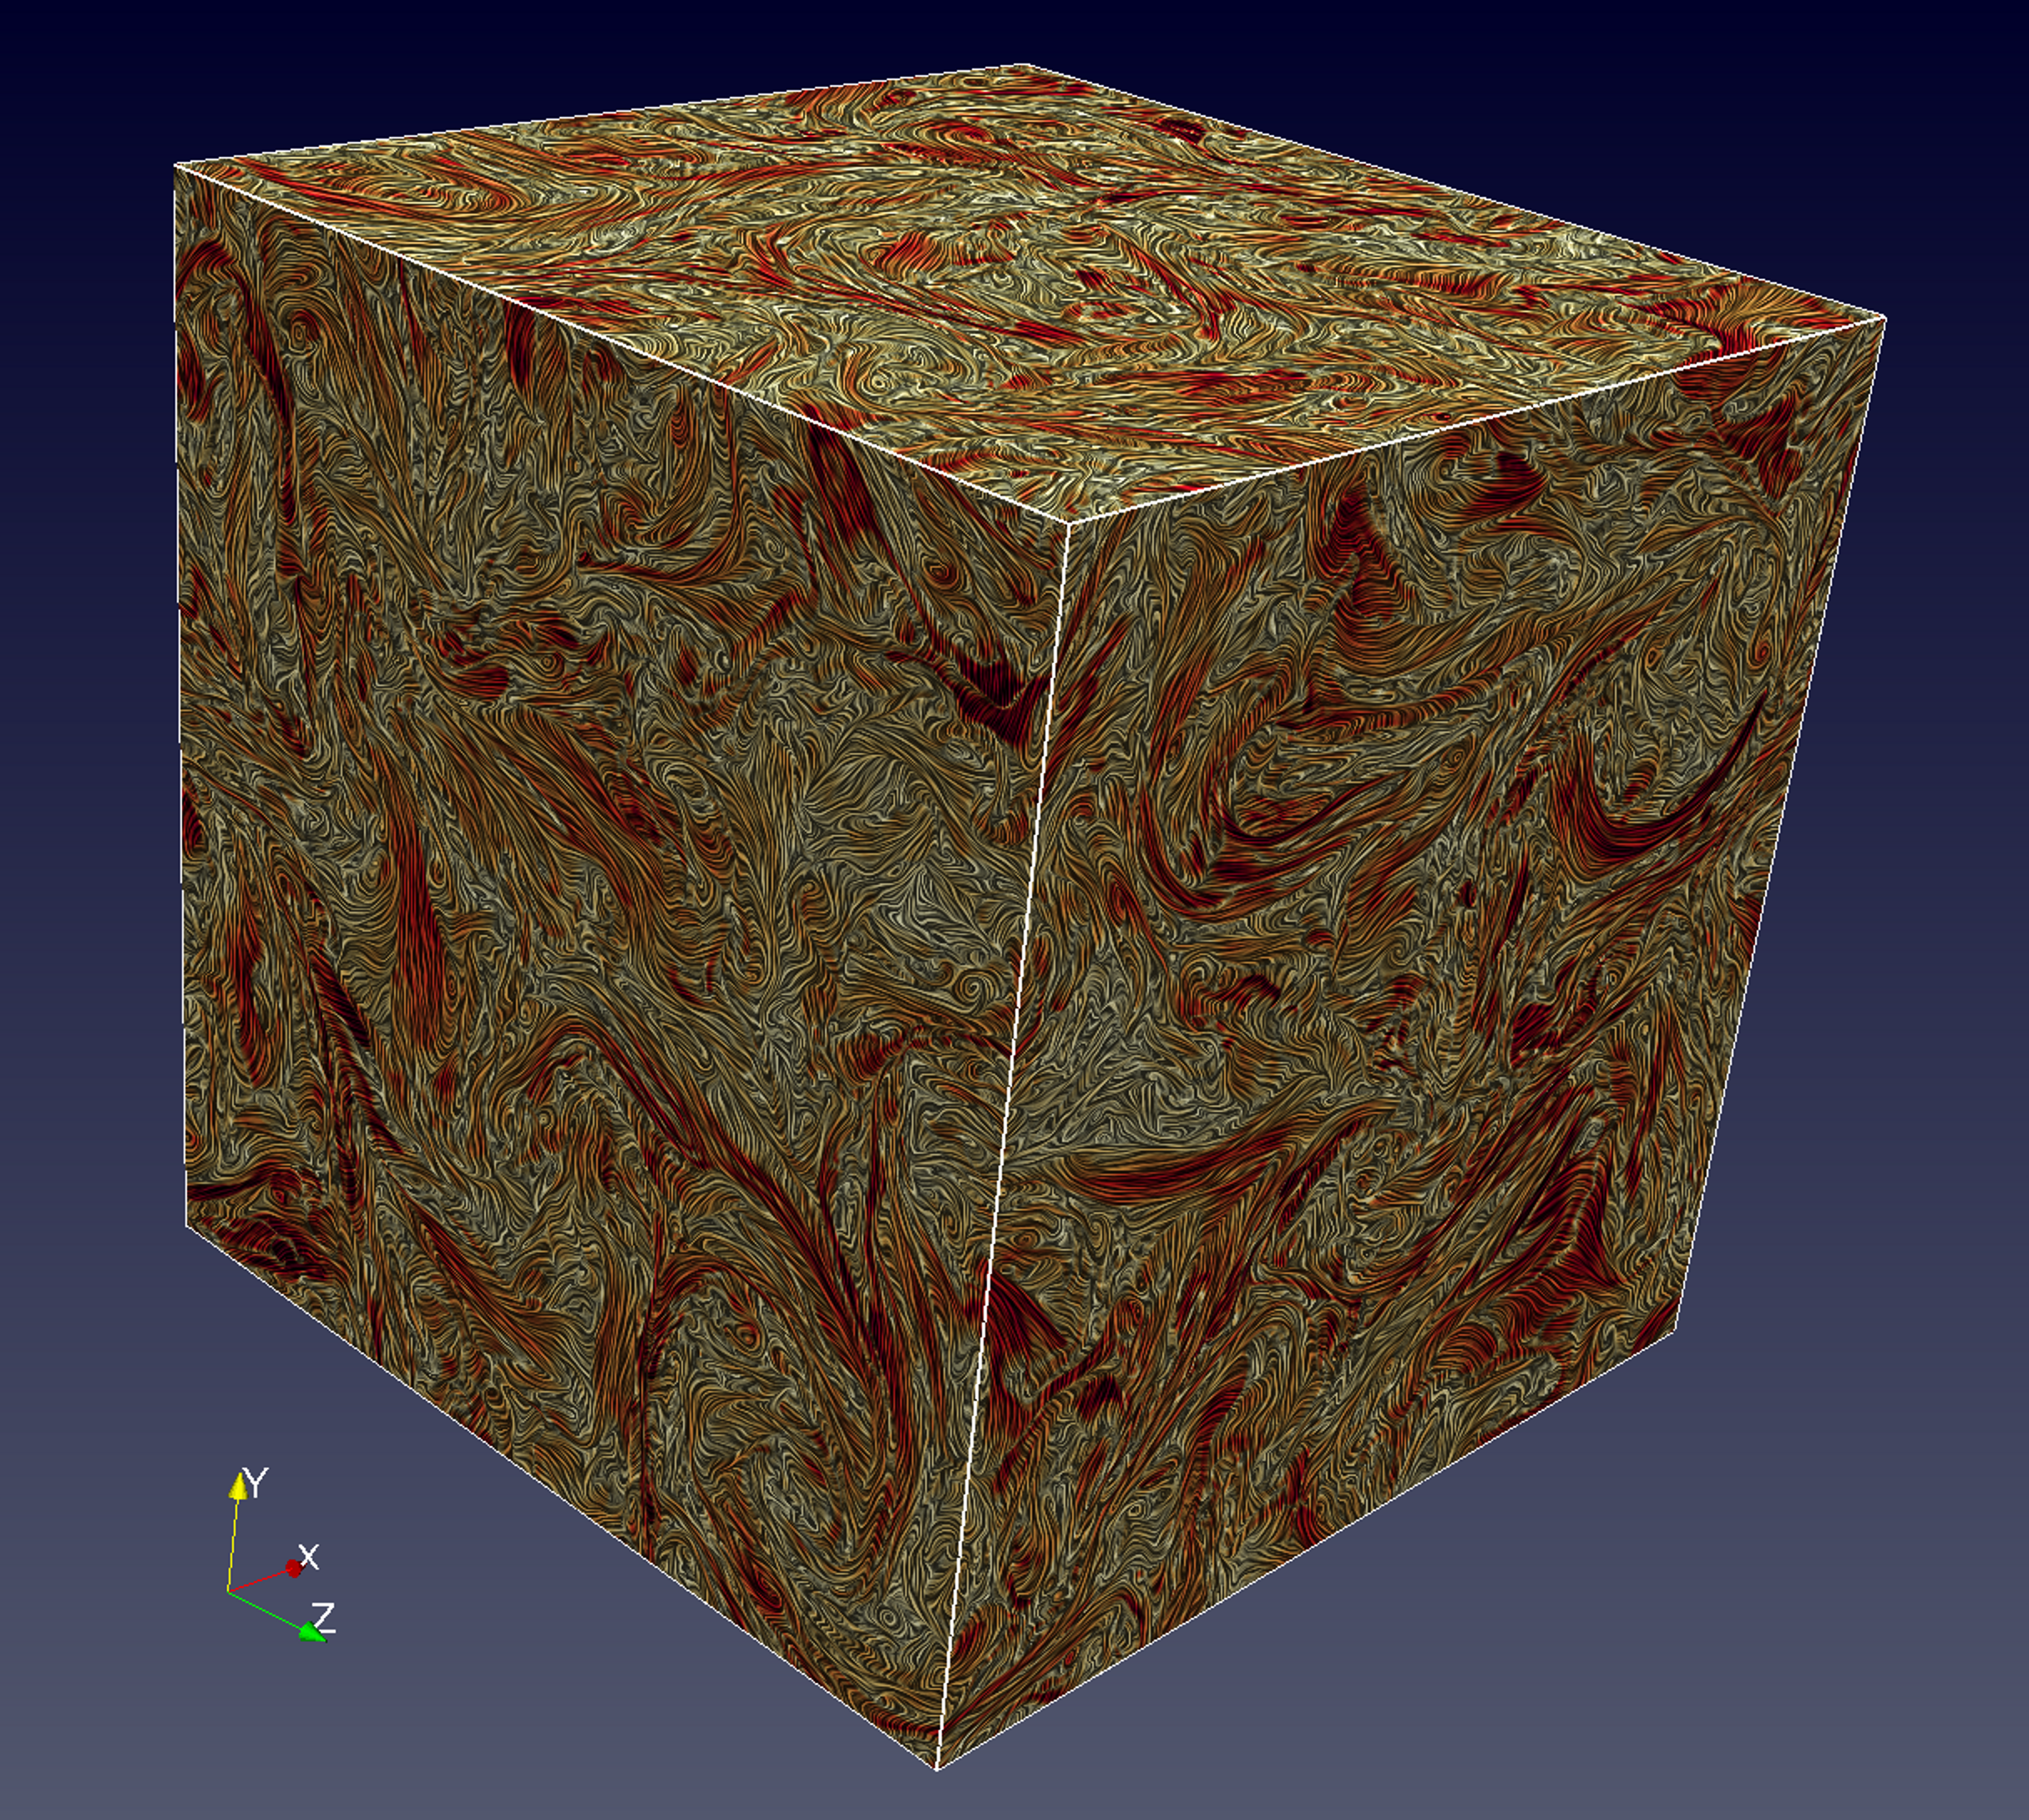
\includegraphics[width=\textwidth]{./images-data/dia-serial/pr1-lic.png}
		% pr1-lic.png: 1215x1090 pixel, 72dpi, 42.86x38.45 cm, bb=0 0 1215 1090
		\label{fig:comp-scaling}  
  \end{subfigure}
\caption{Datasets used for scaling benchmarks. Top: Surface LIC of magnetic field colored by magnitude on the 222M triangle 2D slice Kelvin-Helmholtz turbulent plasma simulation rendered at 2500x1050 px. Bottom: Rendering of the surface LIC of magnetic field colored by magnitude on the $1024^3$ MHD turbulence dataset rendered at 1215x1090 px.}
\end{figure}

\subsection{In-place disjoint strategy}
The main issues with the in-place compositing strategy are that when there is large number of overlap pixels across processes the compositing overhead is high and there is a large amount of redundent computation. These issues can be addressed by making the in-place decomposition disjoint with respect to itself. Figure \ref{fig:pixel-ops} shows an example of how subtraction of extents can produce a disjoint decompositon covering the same area. In that example the extents $\{A-B, B\}$ cover the same areas as $\{A, B\}$ but are disjoint. The in-place domain decomposition can be made disjoint by processing the extents from largest to smallest, taking the largest remaining unprocessed extent and subtracting from it all of the smaller overlaping extents. As each extent is processed it is removed from the list of extents to process and subtract. The set of extents remaining after subraction are added to the new domain decomposition. By definition $A \cap B = B \Rightarrow A - B = B$ therefor processing extents from smallest to largest would result in processes with extents covering others to take ownership of those pixels which could increase work load imbalance. Therefor we process the extents largest to smallest leaving smaller extents in place favoring the preservation of the distribution of work to processes with less work. When the overlap between off process extents is large, compared to the in-place strategy, the in-place disjoint strategy has greatly reduced compositing overhead and redundant computations are eliminated. The intial data distribution is kept in large part because extents in the new domain decomposition automatically remain assigned to the same processes. Note that with the in-place strategy compositing must take place on all processes that overlap of a given region. With the in-place disjoint strategy only one of these processes needs to composite the region. However, when using the in-place disjoint strategy, in order to work with IceT, after the image LIC is computed the result must be transfered back to the original domain decomposition. This is a simple copy rather than a compositing step because the source regions are all disjoint. For this reason equation \ref{eqn:comm-cost} accurately models the number of pixels moved during both composite to and copy from the in-place disjoint decomposition, but is an over estimate of the compositing cost. 

\subsection{Balanced strategy}
\cite{pslic} proposed a 1D domain decomposition of screen space into harizontal strips and load balancing approach that varried the height of the strip such that strips roughly had the same number pixels containing data during the computation. While this would not work well for large tiled displays, one obvious choice for load balancing the image LIC computation in this setting would be to partition the screen into approximately equal sized disjoint 2D patches and assign these uniquely to processes. We briefly investigated this option which we call the ``ballanced'' strategy. The balanced extent partitioner, starting with the tightened view extent, repeatedly divides the new set of pixel extents in half alternating coordinate directions until the desired number of extents is attained. Because the resulting domain decomposition is disjoint by contruction there is no redundant computation. However, the initial distribution of data is not automatically taken into account which may result in unnecessary communication and compositing work, nor is the distribution of work imposed by the new domain decomposition guaranteed to be balanced. In the worst case processes are assigned patches that have no data. To work around the former, a preferential assignment of extents to processes where there is large overlap between the intial and new domain decomposition is needed. To work around the latter, one approach would be to generate more patches than processes and, prior to assigning processes to patches to processes, make a pass over the depth buffer computing the number of pixels that contain data on each extent while culling empty extents. One way to work around this would be  An example of compositing using the balanced decomposition with a single pixel extent per process is shown in figure \ref{fig:compositing} in row 5. Comparing the source and destination decomposition in the first column of row 2 and row 5 it's clear that 

\section{Parallel scaling}
Four sets of scaling benchmarks were made to investigate the scaling performance of the algorithm and compositing strategies with and without GPUs. The runs made investigating the algorithm's performance on GPUs were made on TACC's Longhorn cluster where each compute node is equiped with 48GB RAM, 2 - 4 core 2.5GHz Intel E5540 Nehalem CPUs, 2 NVIDIA Quadro FX 5800 GPUs, and QDR  4 GB/sec Infiniband network. The runs made investigating the algorithms performance without GPUs was made on NERSC's Cray XC30 where each Edison node is equipped with 64GB RAM, 2 - 8 core Intel E5-2670 CPUs, and Cray Aries 8 GB/sec network. On Edison Open GL was provided by Mesa3d 9.2.0 gallium llvmpipe renderer using a per node threading configuration determined in earlier benchmarks\cite{xsede13}.

\begin{figure}[h]
 \centering
\begin{subfigure}{0.45\textwidth}
 \includegraphics[width=1.0\textwidth]{./scaling-ce-slice-gpu.png}
 % scaling-ce-slice-gpu.png: 1600x1200 pixel, 200dpi, 20.32x15.24 cm, bb=0 0 576 432
 \caption{Test of CE scaling on two vector fields}
 \label{fig:ce-scaling}
\end{subfigure}
\hspace{0.1in}
\begin{subfigure}{0.45\textwidth}
 \centering
 \includegraphics[width=1.0\textwidth]{./scaling-composite-cube-gpu.png}
 % scaling-composite-cube-gpu.png: 1600x1200 pixel, 200dpi, 20.32x15.24 cm, bb=0 0 576 432
 \caption{Compositor scaling on MHD turbulence dataset}
 \label{fig:comp-scaling}
\end{subfigure}
\end{figure}

Figure \ref{ce-scaling} shows scaling from 16 to 512 ranks on a massive 16384x8192 VPIC dataset.  The figure shows runs on two vector fields using the settings for a high quality image with and without the new contrast enhancement feature. The figure shows that although the new CE feature makes use of MPI\_Allreduce this does not negatively impact scaling. The differences in performance are attributable to the difference in number of integration steps. Typically I've found that to get the look I want I end up using more integration steps when CE is enabled. A sample image from this run is here: http://www.hpcvis.com/vis/vtk-surface-lic-parallelization/kh-new-jaguar-lic-b-woce.png

Figure \ref{comp-scaling} show scaling from 16 to 512 ranks on a large $1204^3$ MHD turbulence dataset and a comparison of two of the compositing algorithms. The INPLACE option is what you and I had initially discussed on Skype, while the INPLACE\_DISJOINT option ensures that each fragment is computed only once by uniquely assigning ownership of regions of the screen to ranks while leaving the data in-place ie. a rank doesn't take ownership of a fragments it doesn't have data for. For the INPLACE\_DISJOINT approach the compositing communication cost is the same or in some cases less than the INPLACE approach although it's split into two phases(gather and scatter). The figure shows that the INPLACE\_DISJOINT method offers a nice increase in performance. The speed up is larger in the smaller runs because in those runs the screen regions by rank are larger, and this presents a greater opportunity to reduce the number of fragments processed per rank. The following teo plots show this better. The image produced by these runs is here: http://www.hpcvis.com/vis/vtk-surface-lic-parallelization/pr1-lic.png

\begin{figure}[h]
 \centering
 \includegraphics[width=1.0\textwidth]{./scaling-gant-inplace-composite-gpu-mesa.png}
 % scaling-gant-inplace-composite-gpu-mesa.png: 2046x1095 pixel, 200dpi, 25.98x13.91 cm, bb=0 0 737 394
 \caption{INPLACE Compositing}
 \label{fig:inplace-comp}
\end{figure}

These two figures are Gant plots of each rank's activity during the 2 node 16 rank compositing INPLACE and INPLACE\_DISJOINT scaling runs. We're looking at the 2-node case because it shows the greatest speed up for the INPLACE\_DISJOINT compositor and it will be easier to see the performance differences between the two. For both runs most of the time is spent in RenderGeometry (vector projection and light vertex shaders) and Integrate1/Integrate2 phases. CE phases tend to look long because of the MPI\_Allreduce ranks get synchronized by the slowest rank so most of the time spent there is waiting. The RenderGeometry and GatherVectors(compositing and guard pixel exchange) times are nearly identical for both compositors. This means that speed up attained by the INPLACE\_DISJOINT compositor is a result of reduced integration time while computing the LIC. With INPLACE\_DISJOINT approach each rank has fewer fragments to process and there's a greater opportunity to cull empty fragments as the screen space regions are decomposed. These plots also show that the overhead of decomposing(makiing the screenspace disjoint amongst ranks) is small enough to be negligible and that although the INPLACE\_DISJOINT moves less data around during compositing and guard pixel exchange it doesn't contribute a lot to the speed of the approach.

\begin{figure}[h]
 \centering
 \includegraphics[width=1.0\textwidth]{./scaling-gant-inplace-disjoint-composite-gpu-mesa.png}
 % scaling-gant-inplace-disjoint-composite-gpu-mesa.png: 2128x1096 pixel, 200dpi, 27.03x13.92 cm, bb=0 0 766 395
 \caption{DISJOINT Compositor}
 \label{fig:disj-comp}
\end{figure}

For example the perfromance difference between inplace and inplace disjoint decompositon in figure \ref{fig:comp-scaling}. This can be seen by comparing the compositing and integration times reported in figure \ref{fig:inplace-comp} with those reported in \ref{fig:disj-comp}.





\FloatBarrier

\section{Apendix A}
\label{sec:pslic-outputs}
\begin{figure}[h]
	\centering
	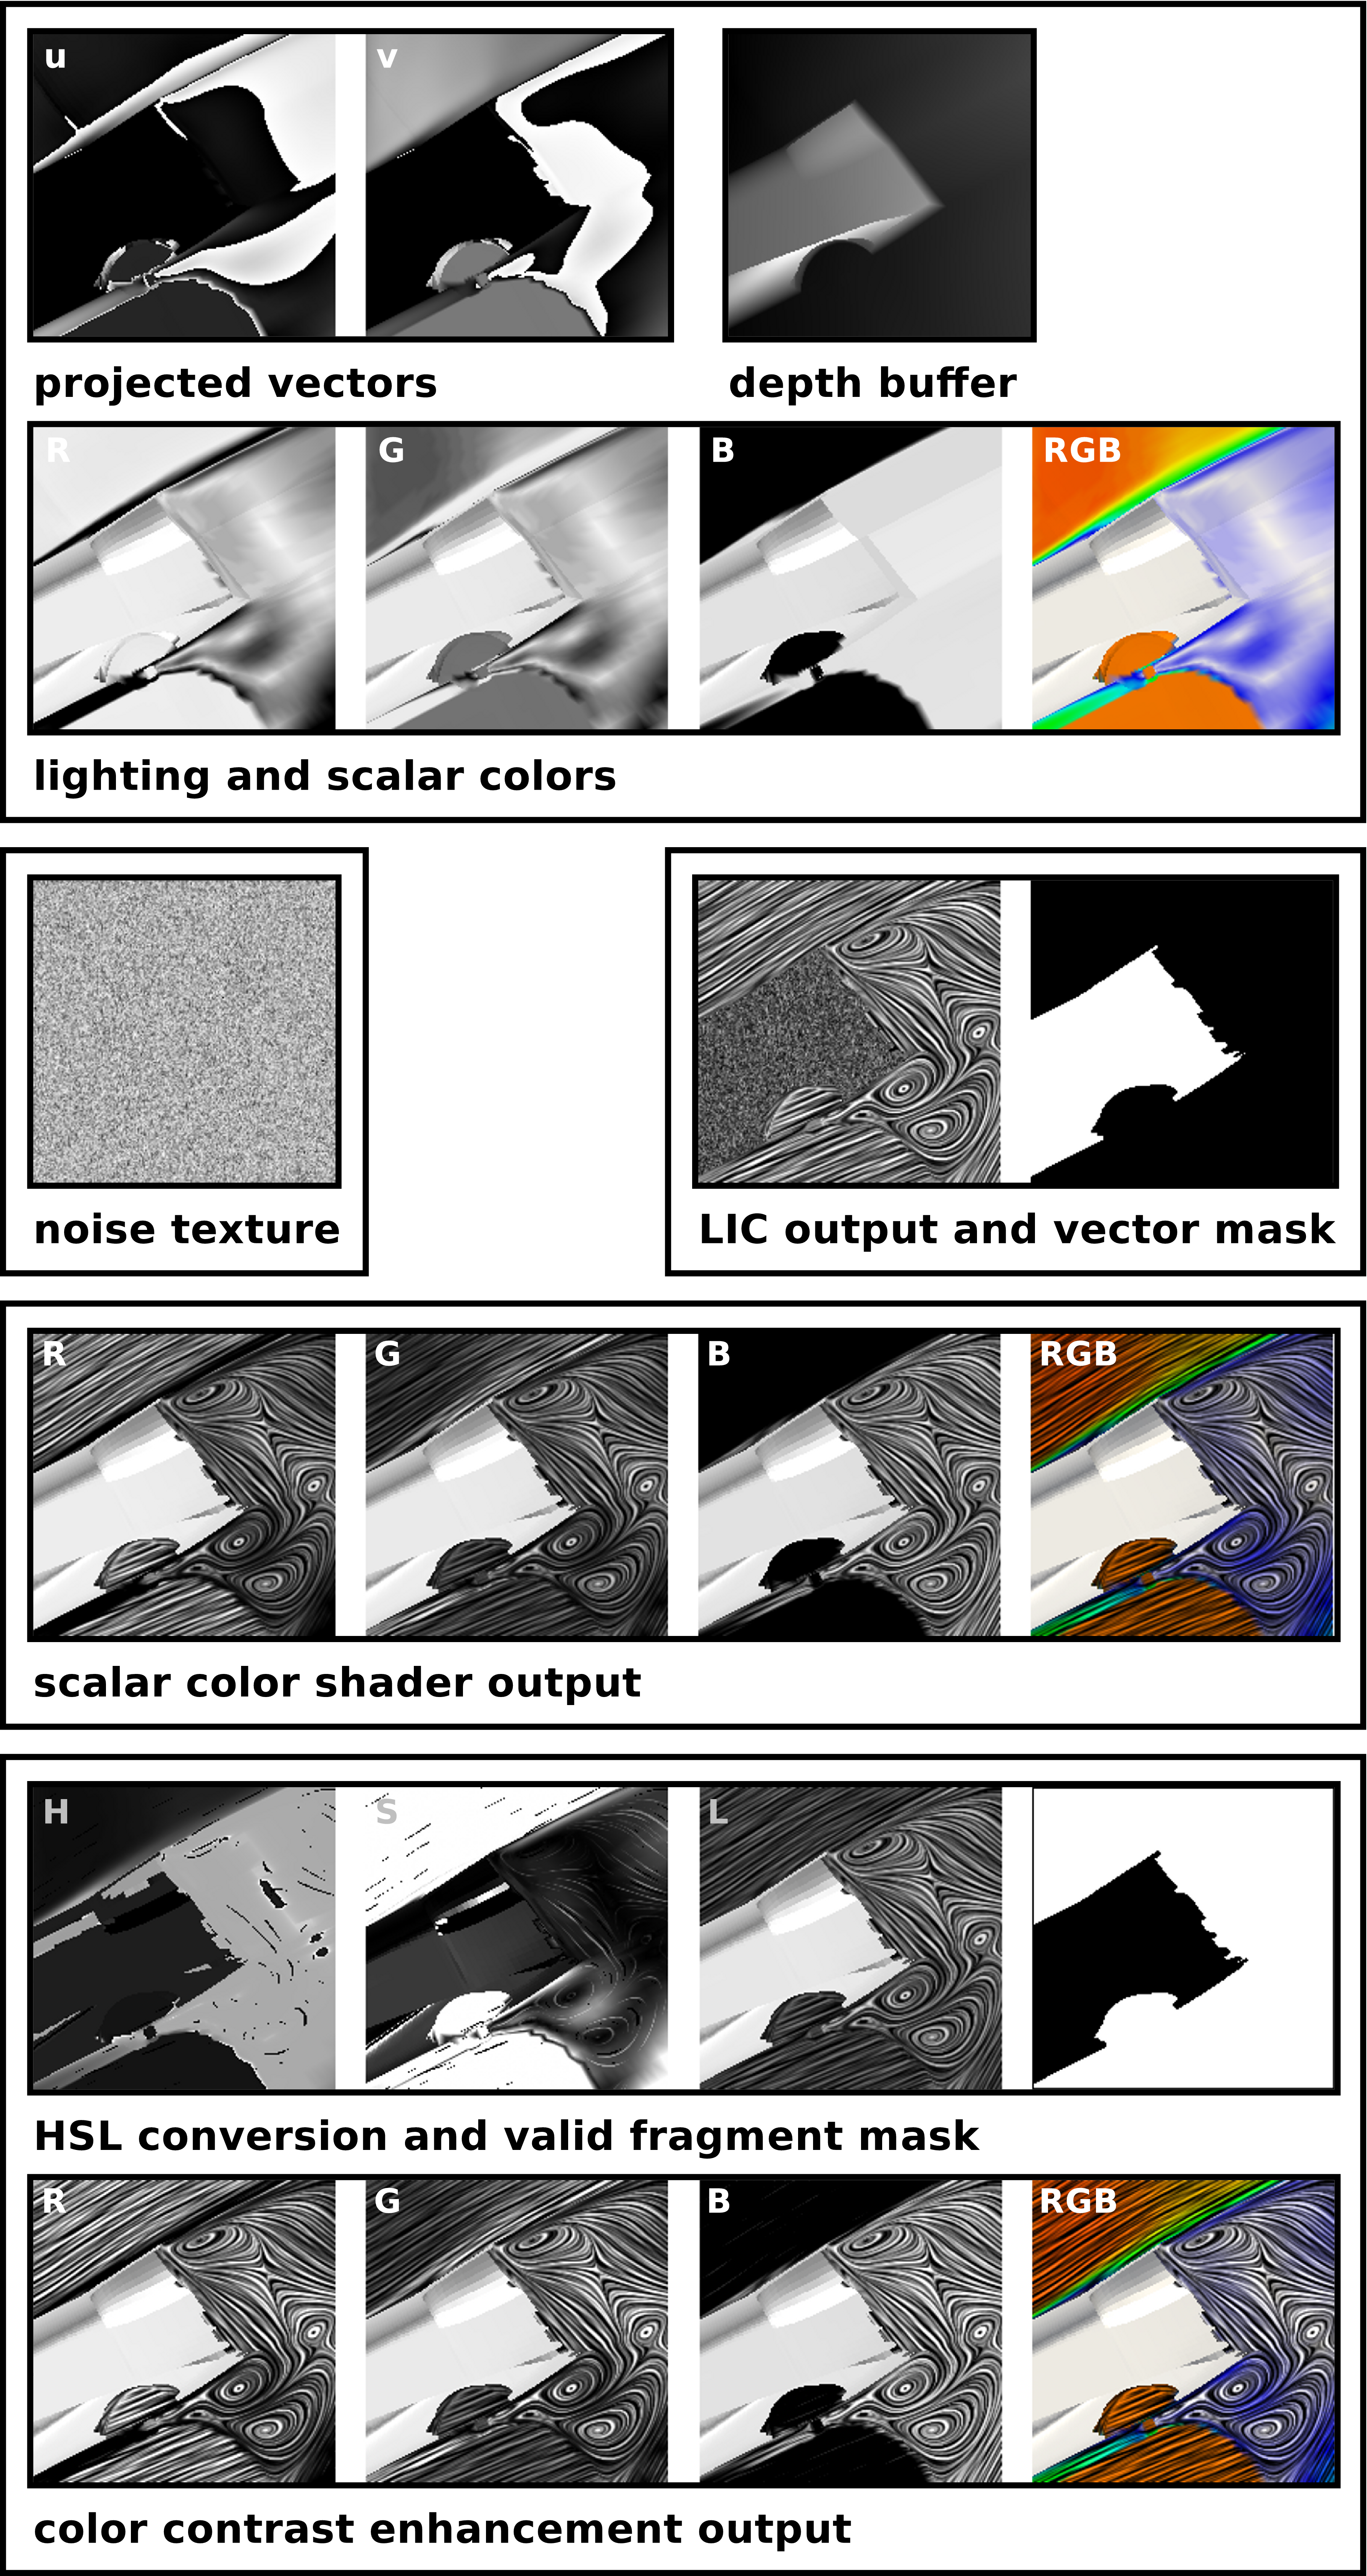
\includegraphics[width=0.75\textwidth]{./images-data/dia-serial/lg-surface-lic-painter-200ppi.png}
	\label{fig:lic2d-outputs}
  \caption{Outputs from the logical processing stages of our surface LIC algorithm. See figure \ref{fig:flow} for the stages.}
\end{figure}
\FloatBarrier

% \section{Appendix B}
% \label{sec:scaling-data}
% \begin{figure}[h!]
%  \centering
%  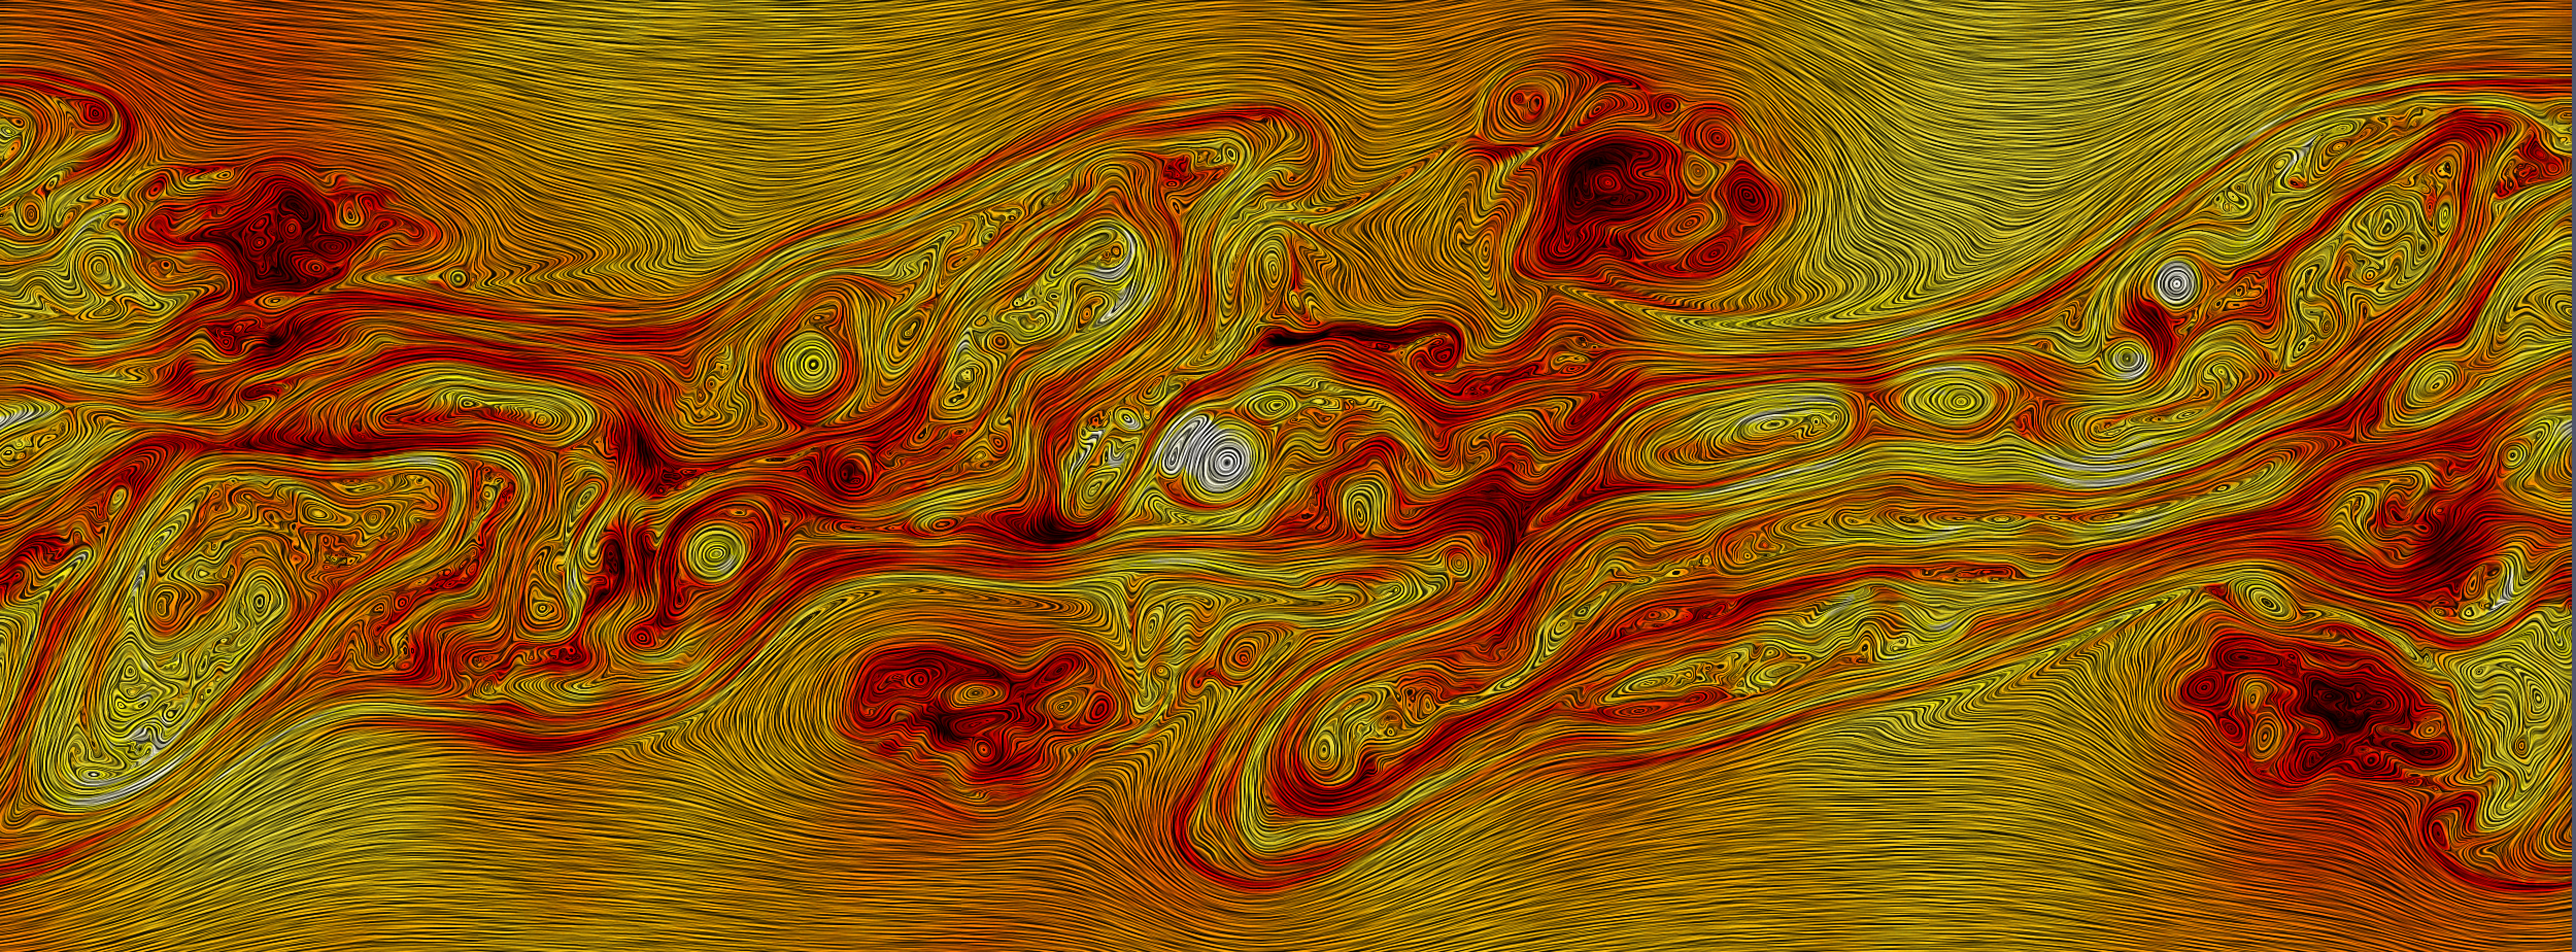
\includegraphics[width=0.9\textheight,angle=90]{./images-data/dia-serial/lic-b-427-hr.png}
%  % lic-b-427-hr.png: 5000x1848 pixel, 72dpi, 176.37x65.19 cm, bb=0 0 4999 1848
%  \caption{Rendering of the 222M triangle slice dataset used for scaling runs.}
%  \label{fig:scaling-lic}
% \end{figure}
% 
% \begin{figure}[ht]
%  \centering
%  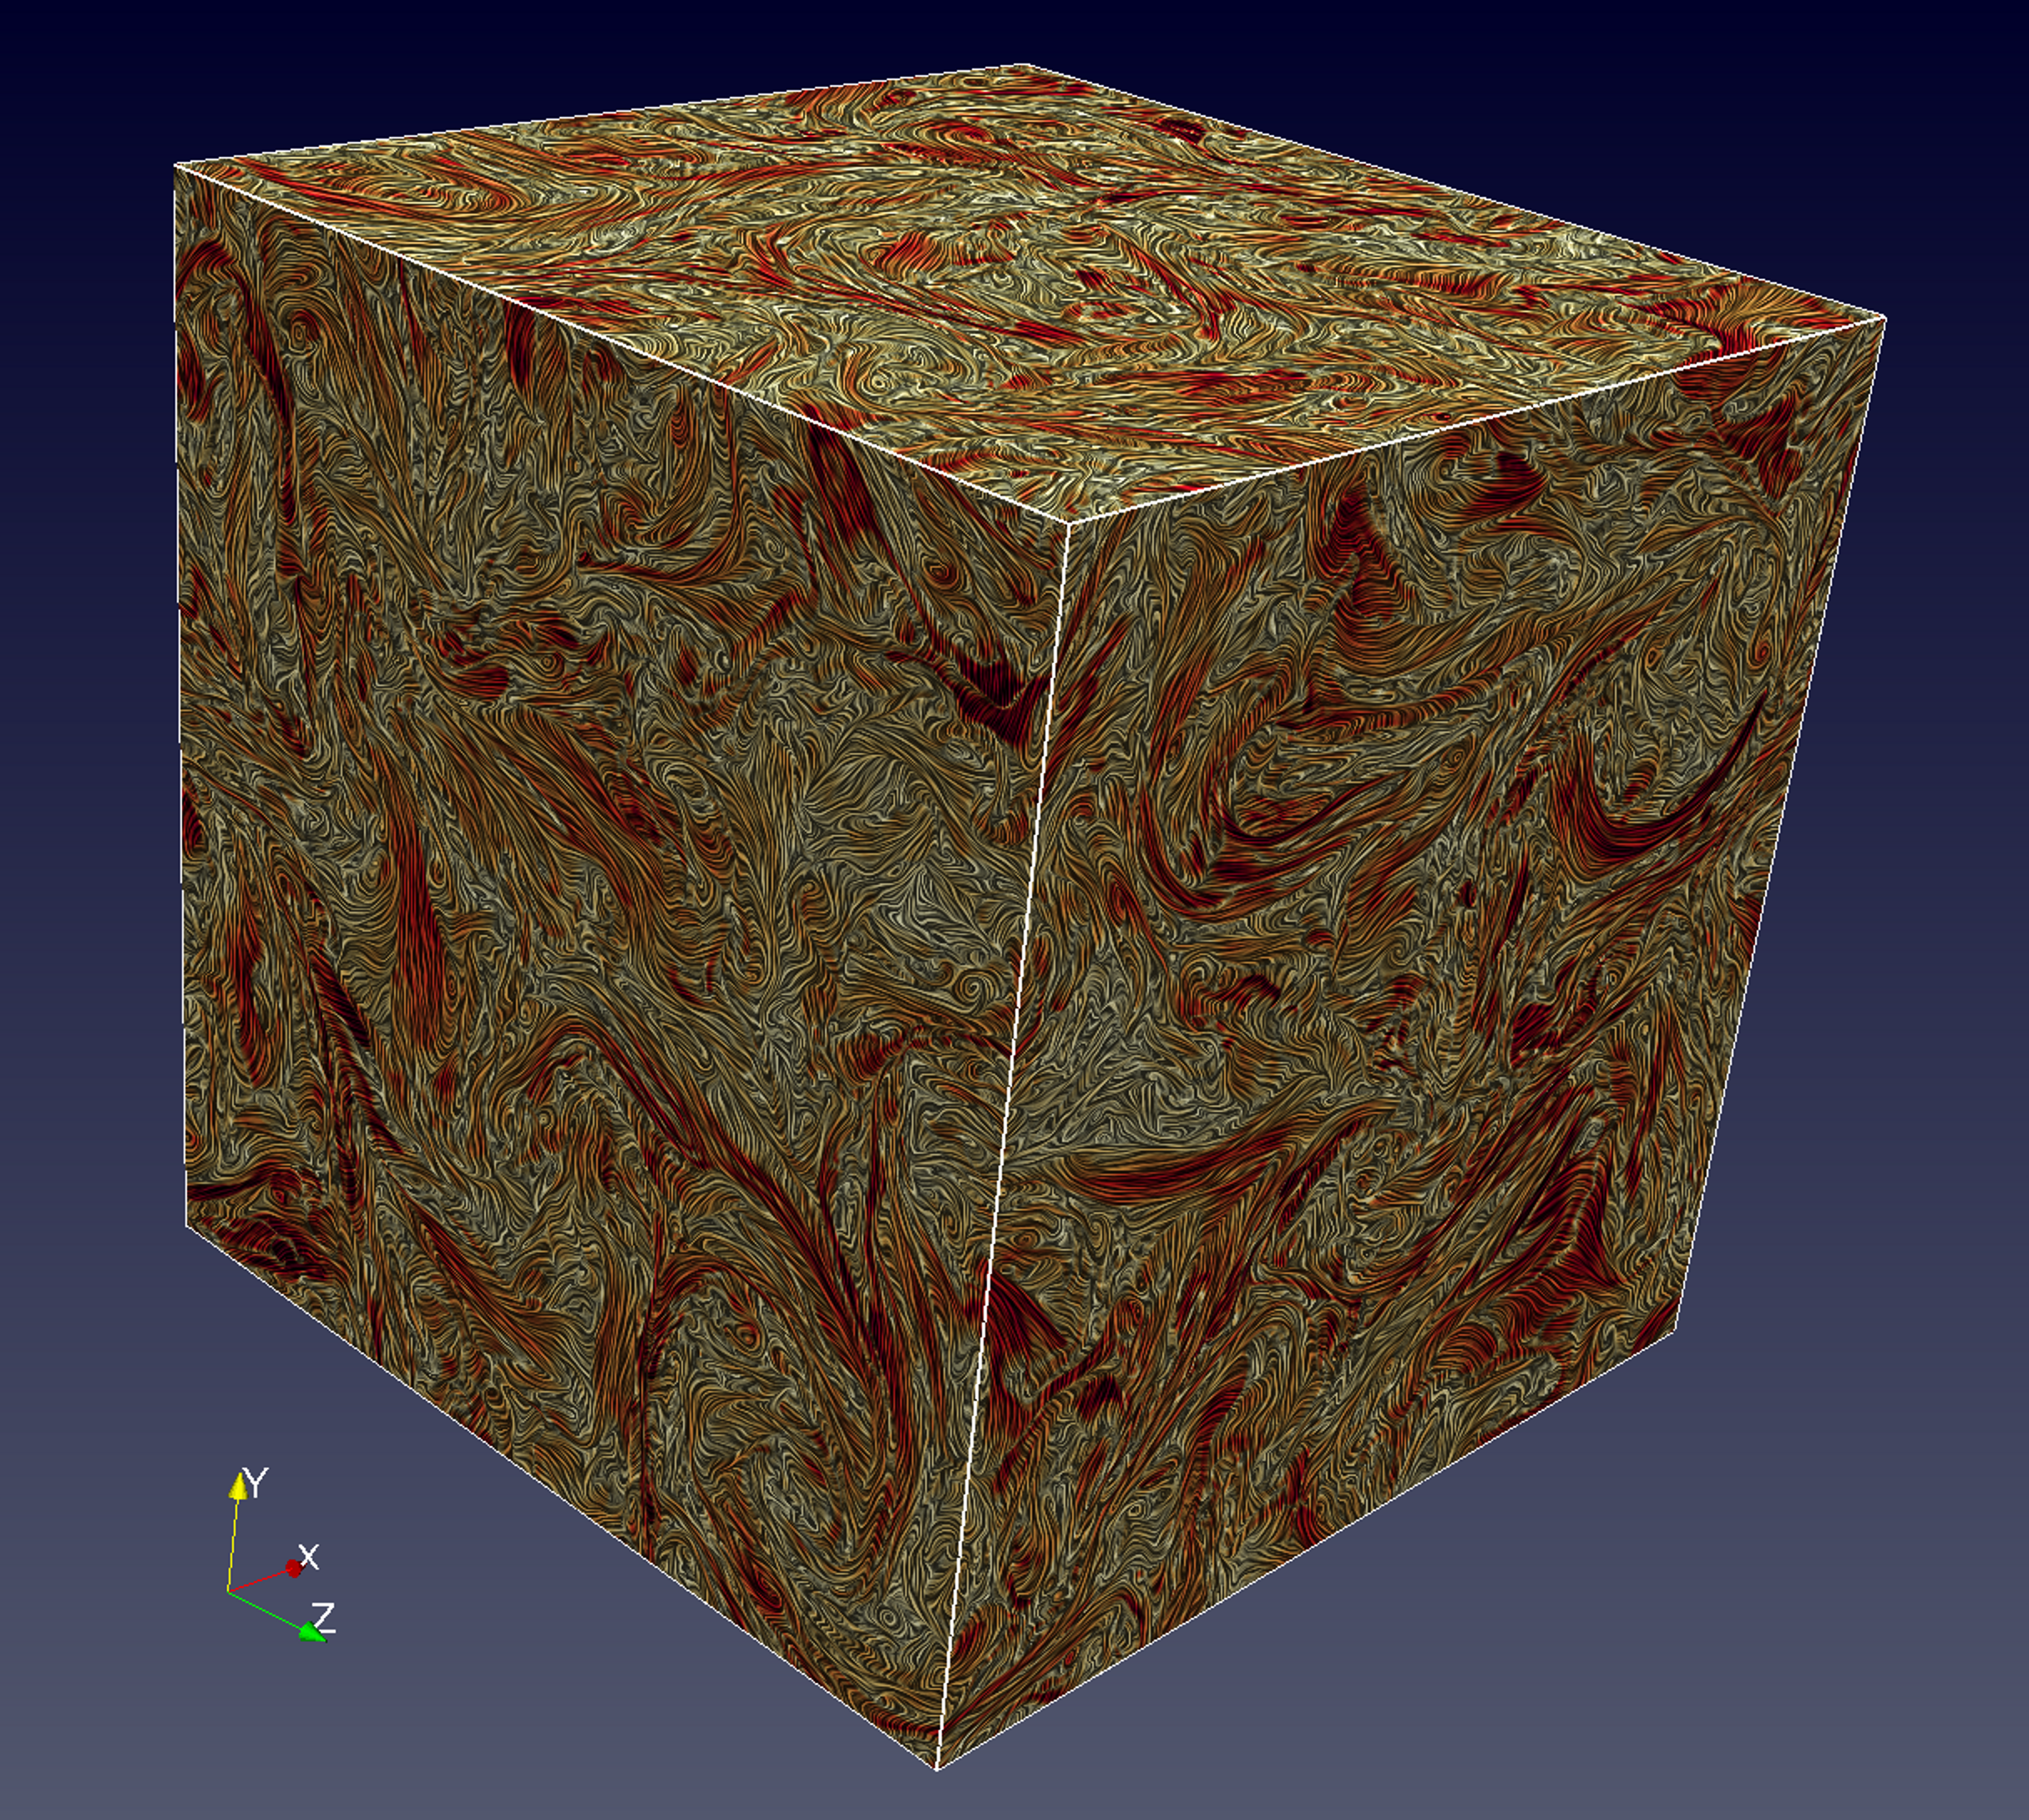
\includegraphics[width=\textwidth]{./images-data/dia-serial/pr1-lic.png}
%  % pr1-lic.png: 1215x1090 pixel, 72dpi, 42.86x38.45 cm, bb=0 0 1215 1090
%  \caption{compositor scaling test data}
%  \label{fig:comp-scaling}
% \end{figure}


% shuttle launch vehicle dataset
% P.G. Buning, I.T. Chiu, F.W. Martin, Jr., R.L. Meakin, S. Obayashi, Y.M. Rizk, J.L. Steger, and M. Yarrow, "Flowfield Simulation of the Space Shuttle Vehicle in Ascent," Fourth International Conference on Supercomputing, Vol II, Supercomputer Applications, Kartashev & Kartashev, eds., 1989, pp. 20-28.


\section{Appendix C}
\begin{figure}[h]
 \centering
 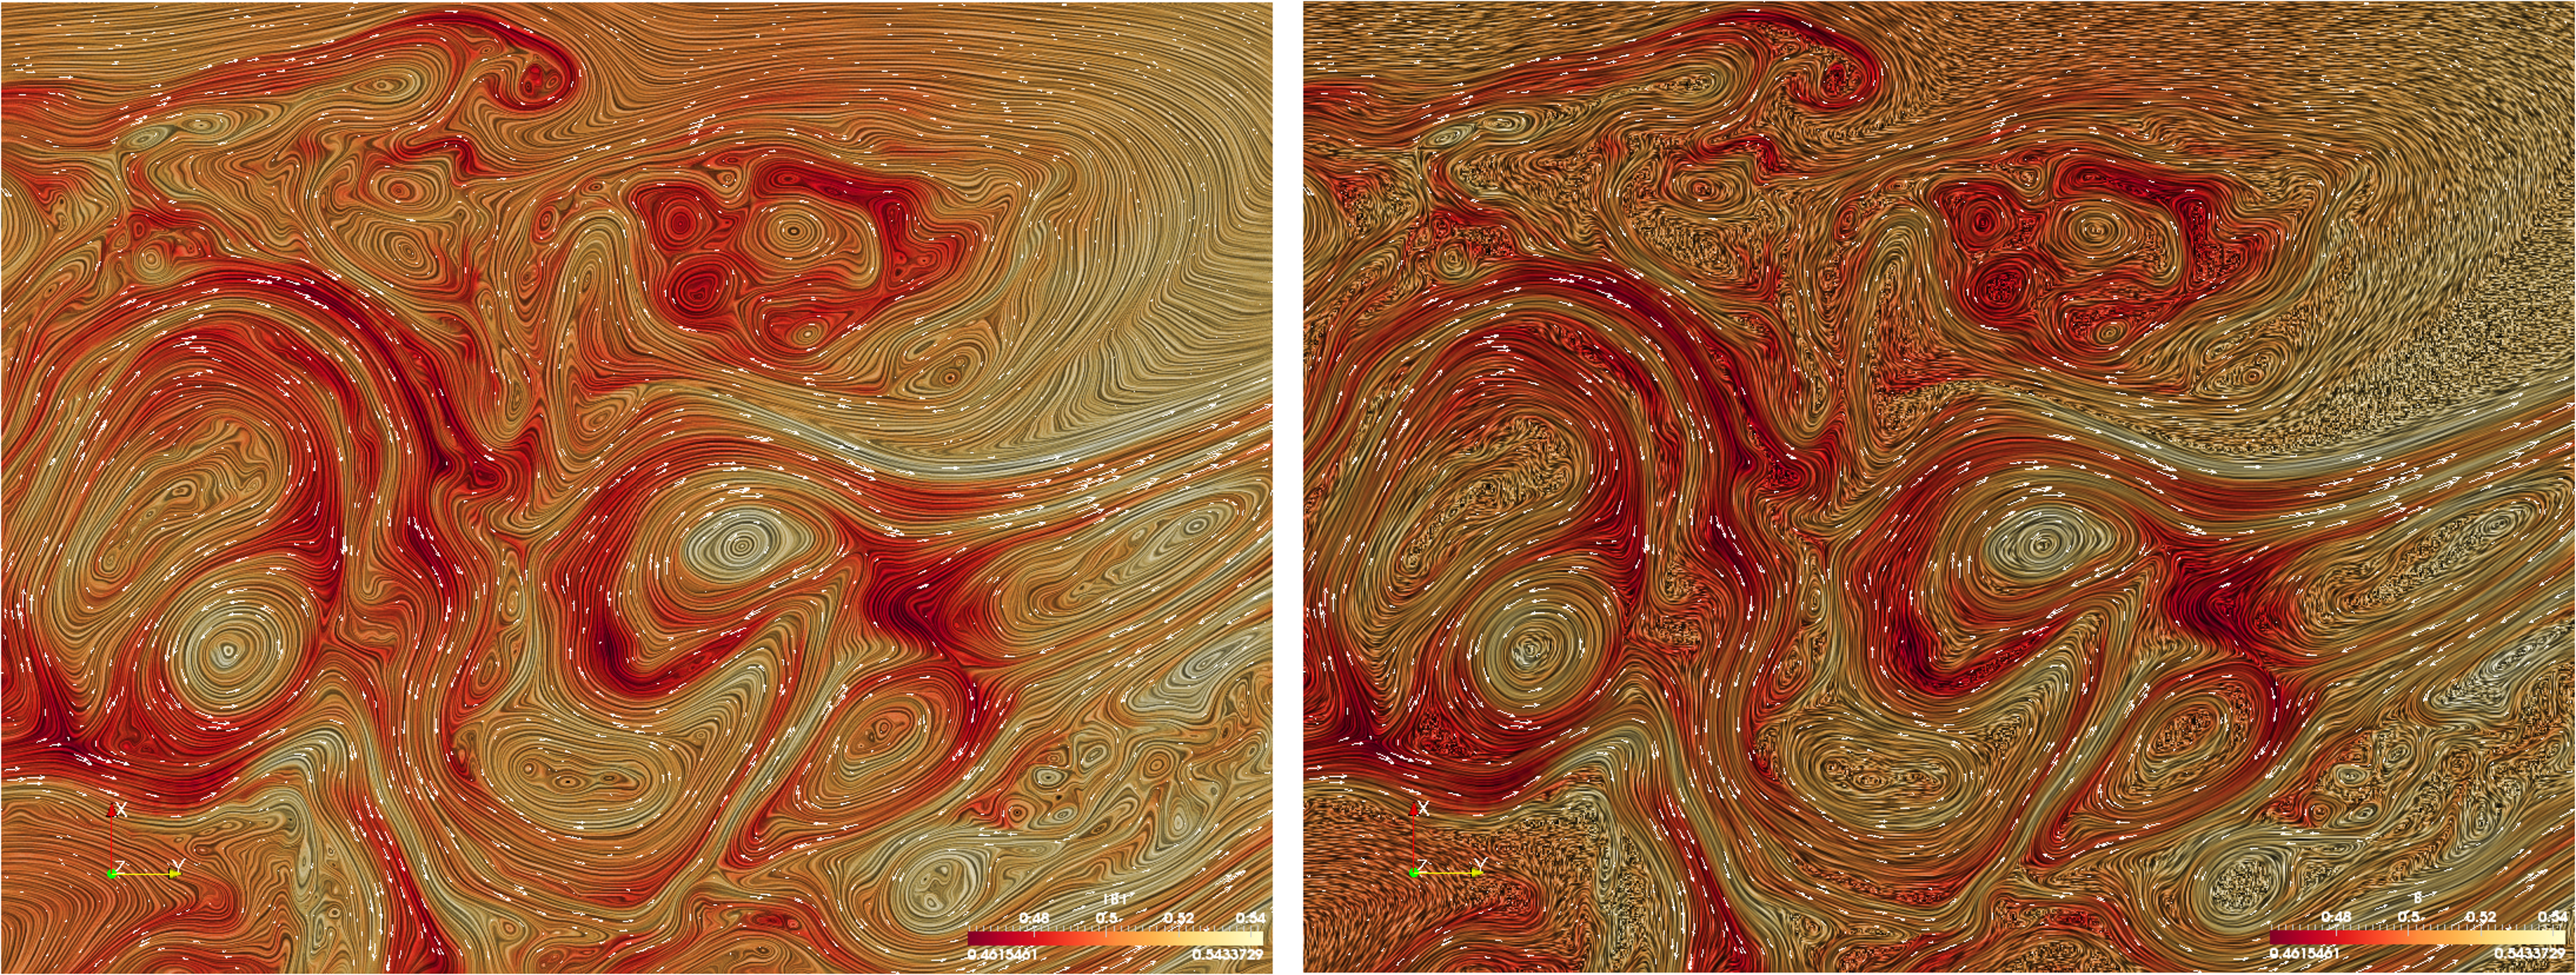
\includegraphics[width=\textwidth]{./images-data/dia-serial/kh-b-norm-vs-no-norm.png}
 % kh-b-norm-vs-no-norm.png: 4376x1656 pixel, 72dpi, 154.36x58.41 cm, bb=0 0 4375 1656
 \caption{Integrator normalization}
 \label{fig:vec-norm-2}
\end{figure}

\section{Appendix D}
\begin{figure}[h]
 \centering
 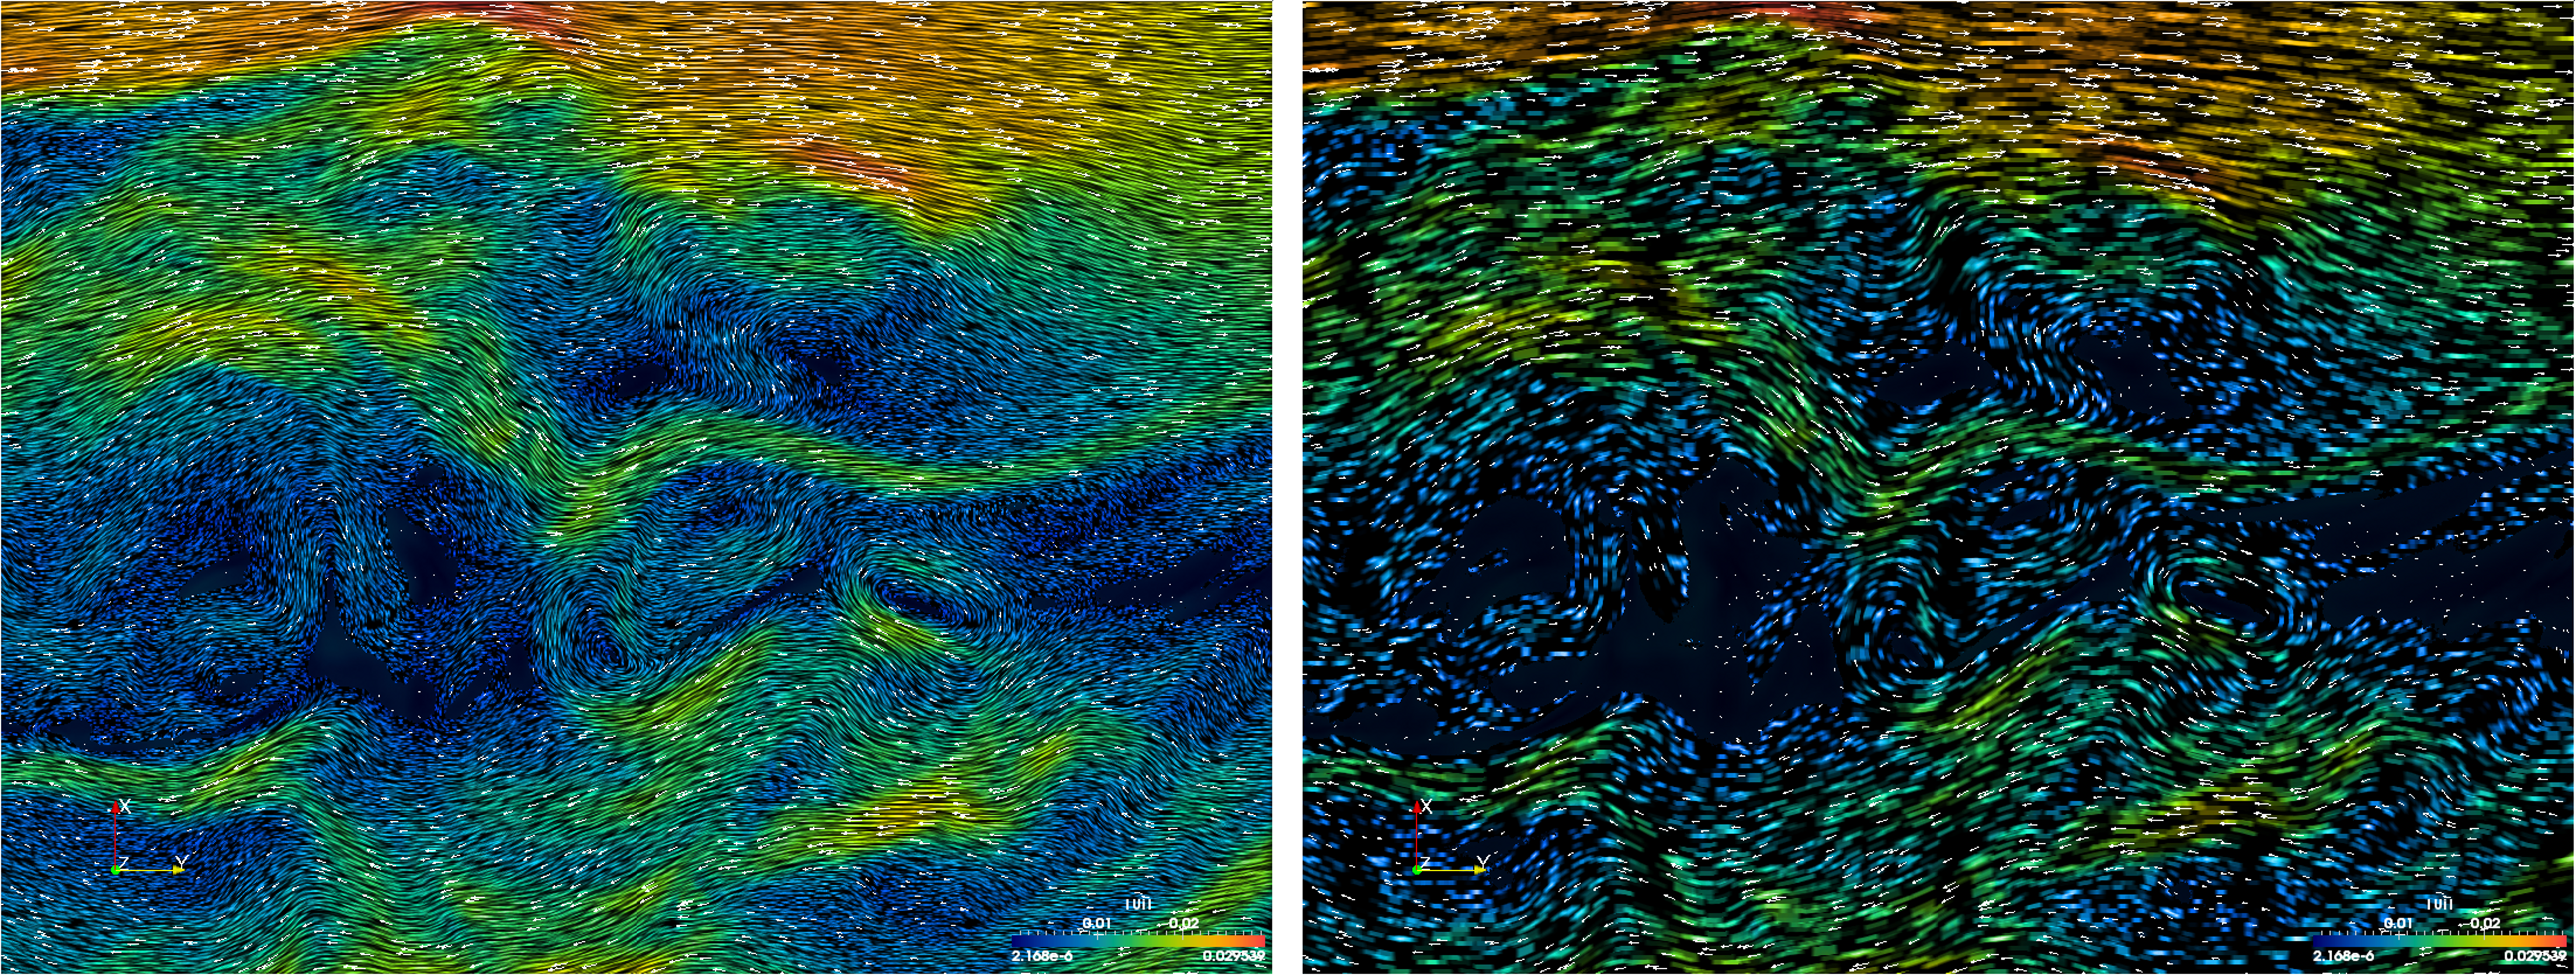
\includegraphics[width=\textwidth]{./images-data/dia-serial/kh-ui-with-varying-noise.png}
 % kh-ui-with-varying-noise.png: 4410x1670 pixel, 72dpi, 155.56x58.91 cm, bb=0 0 4409 1670
 \caption{Noise texture generator parameters}
 \label{fig:noise-params}
\end{figure}

\section{Appendix E}
\begin{figure}[ht]
 \centering
 \includegraphics[width=\textwidth]{./images-data/dia-serial/various-noise-shader.png}
 % various-noise-shader.png: 1230x1229 pixel, 72dpi, 43.39x43.35 cm, bb=0 0 1230 1229
 \caption{various combinations of custom noise and shader}
 \label{fig:various}
\end{figure}

\section{Appendix F}
\begin{figure}[ht]
 \centering
 \includegraphics[width=0.9\textwidth]{./images-data/dia-serial/ex-blow-balanced-screen-exts-guard-pixels-ddepth-all.png}
 % ex-blow-balanced-screen-exts-guard-pixels-ddepth-all.png: 887x522 pixel, 72dpi, 31.29x18.41 cm, bb=0 0 887 522
 \caption{balanced domain decomp, in balanced work load.}
 \label{fig:balanced-bad}
\end{figure}


\end{document}